\documentclass{article}
\usepackage{ctex}
\usepackage{geometry}
\usepackage{fancyhdr}
\usepackage{zhlipsum}
\usepackage{lastpage}
\usepackage{float}
\usepackage{graphicx}
\usepackage{paralist}
\usepackage{booktabs}
\usepackage{fancybox}
\usepackage{hyperref}
\usepackage{listings}
\usepackage{xcolor}

\let\itemize\compactitem
\let\enditemize\endcompactitem
\let\enumerate\compactenum
\let\endenumerate\endcompactenum
\let\description\compactdesc
\let\enddescription\endcompactdesc

\geometry{a4paper,left=25mm,right=20mm,top=25mm,bottom=25mm}

\lstset{
    numbers=left,
    keywordstyle= \color{ blue!70},
    commentstyle= \color{red!50!green!50!blue!50},
    rulesepcolor= \color{ red!20!green!20!blue!20} ,
    escapeinside=``,
    numberstyle=\tt,
    numbersep=1em,
    xleftmargin=2em,
    breaklines,
    aboveskip=1em,
    framexleftmargin=3em,
    frame=shadowbox,
    basicstyle=\tt,
    language=Java
}


\title{虚拟校园系统使用说明书}

\begin{document}

\begin{titlepage}
  \vspace*{\fill}

  \begin{center}
    {\Huge 虚拟校园系统使用说明书}

    \vspace{10cm}
    {\large
      09021227~金\phantom{金}桥 \\
      09021218~马晓龙 \\
      09021134~王智东 \\
      09021130~张博雅 \\
      09021202~钟世贵 \\
      09021215~曹江宁
    }

    \vspace{0.5cm}
    {\large 版本:\texttt{1.0.0-release}}


    \vspace{0.5cm}


    {\large 日期:\today}
  \end{center}

  \vspace*{\fill}
\end{titlepage}
\tableofcontents
\newpage

\section{前言}

本文档为东南大学2021级计算机科学与技术专业暑期实训vCampus项目客户端使用说明书。

\section{使用说明}
\subsection{登录}

\begin{center}
\shadowbox{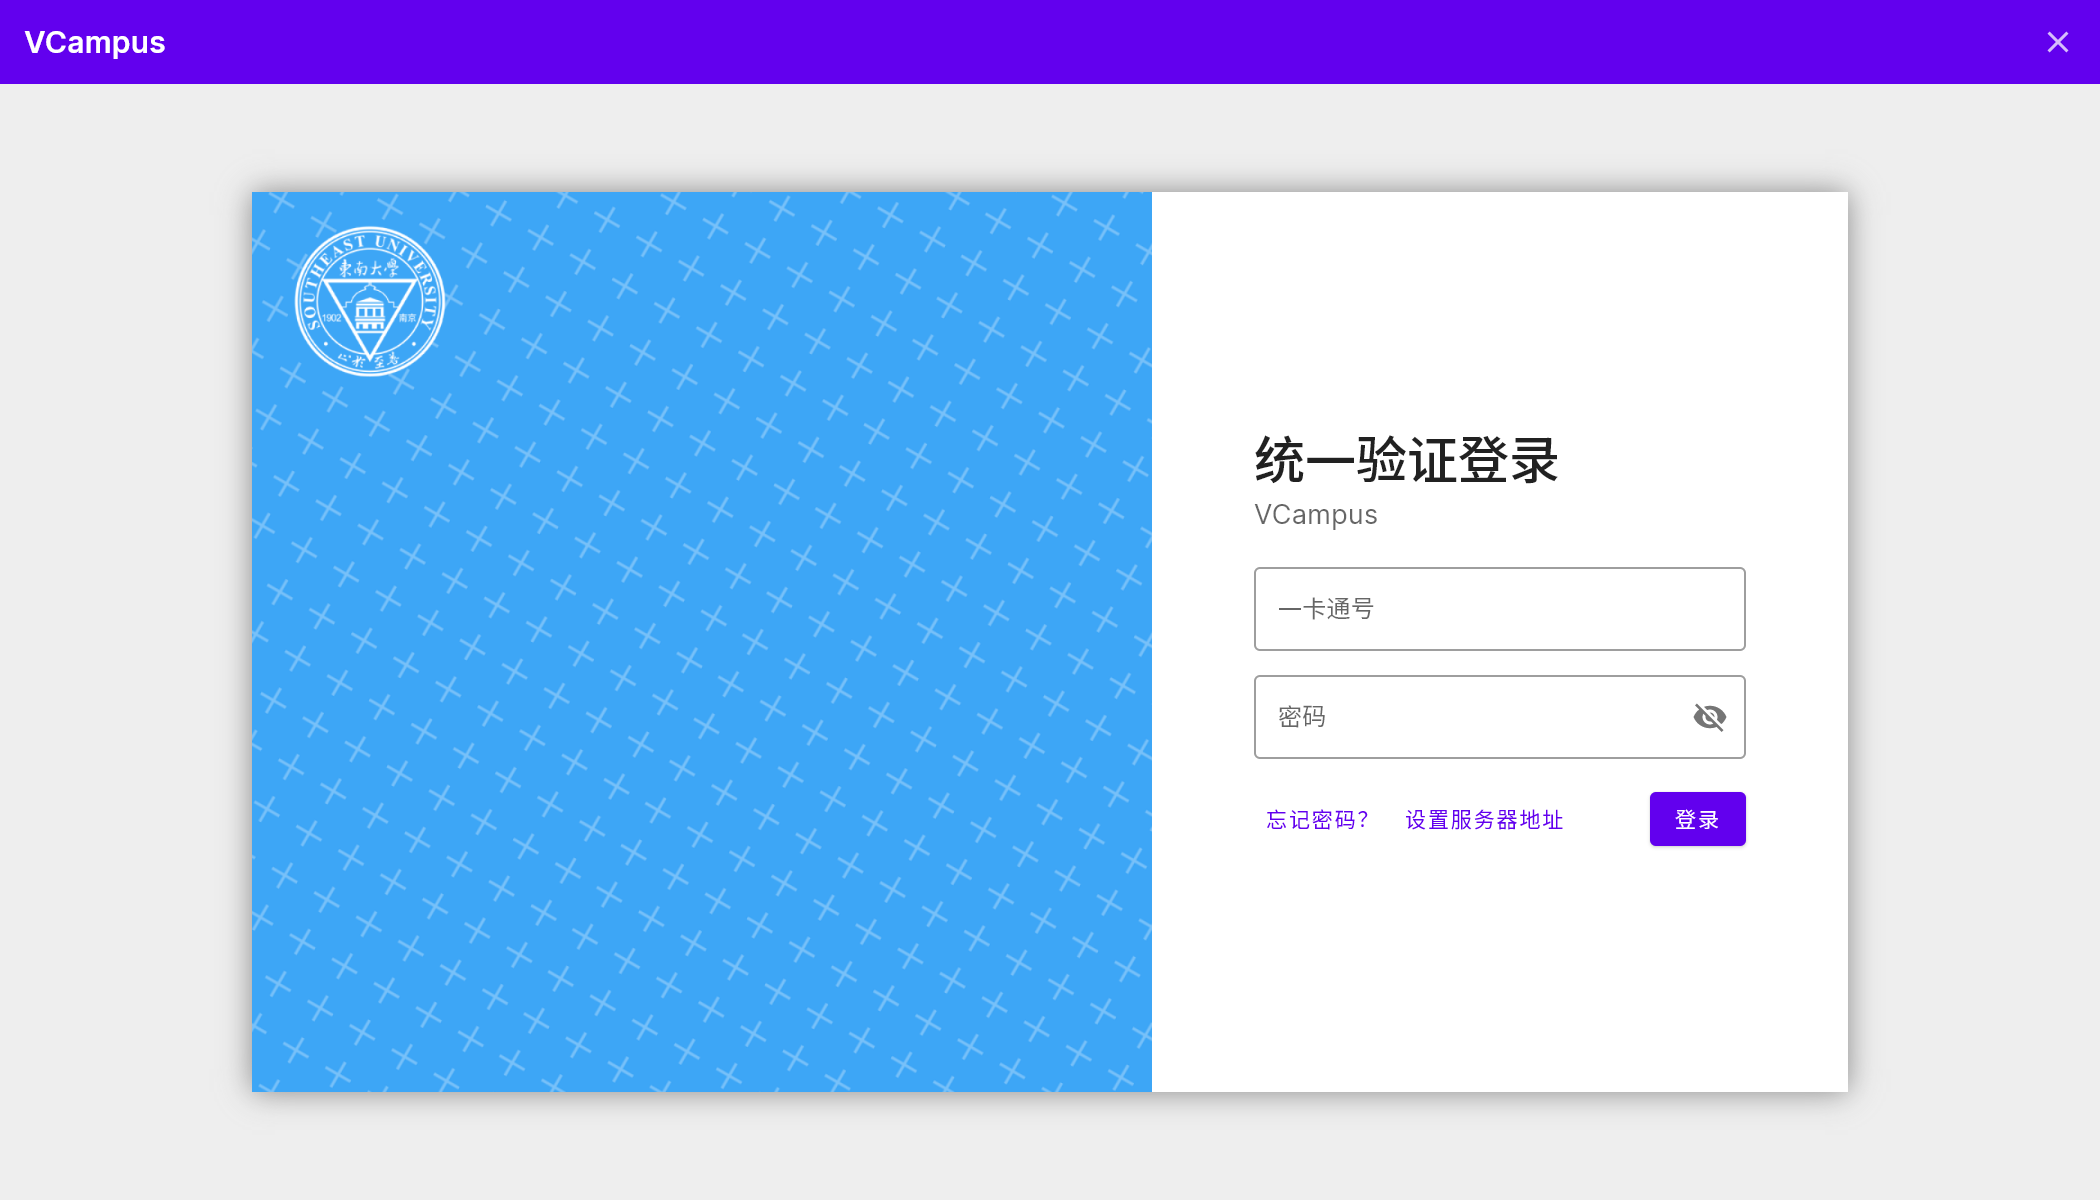
\includegraphics[width=\textwidth]{fig/login/login.png}}
\textbf{登录界面}
\end{center}

\subsection{学籍}

\subsubsection{我的学籍信息}
该界面为学生登录vcampus后在教务工具栏进入所显示的界面,在我的学籍信息界面中,学生可以查看自己目前的个人学籍信息,其中包括自己的姓名,性别,学院名称,专业名称,一卡通号,学号等基础信息。

\begin{center}
\shadowbox{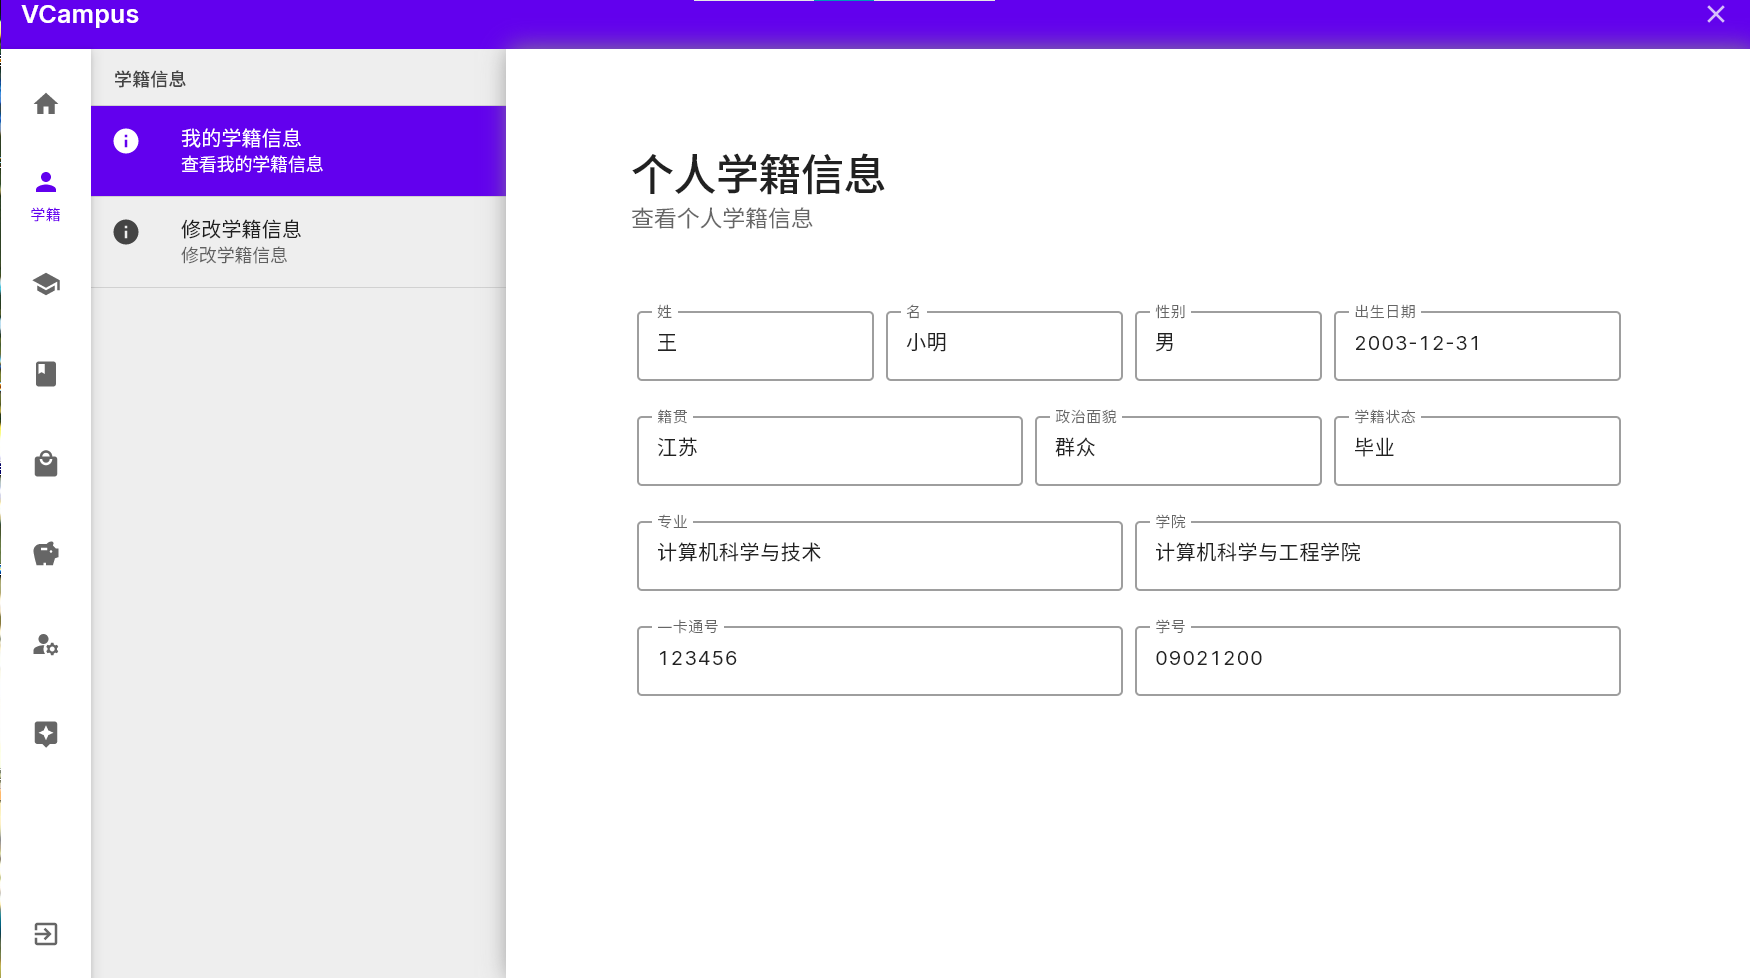
\includegraphics[width=\textwidth]{fig/student_status/student-status-show.png}}
\textbf{我的学籍信息界面}
\end{center}

\subsubsection{修改学籍信息}
该界面为学籍信息管理人员登录vcampus后在教务工具栏进入后所显示的界面,在这个界面中,我们提供了一个搜索框,你可以输入姓名、一卡通号、学号等信息进行相关学术的索引。如果你希望查看现在所有的学术学籍信息,可以在搜索框为空时进行搜索,此时系统会加载显示所有的学生学籍信息。同时,查询得到对应学生的学籍信息后,你可以点击查看详情,并且根据按钮提示进行相关学籍信息的修改。
\begin{center}
\shadowbox{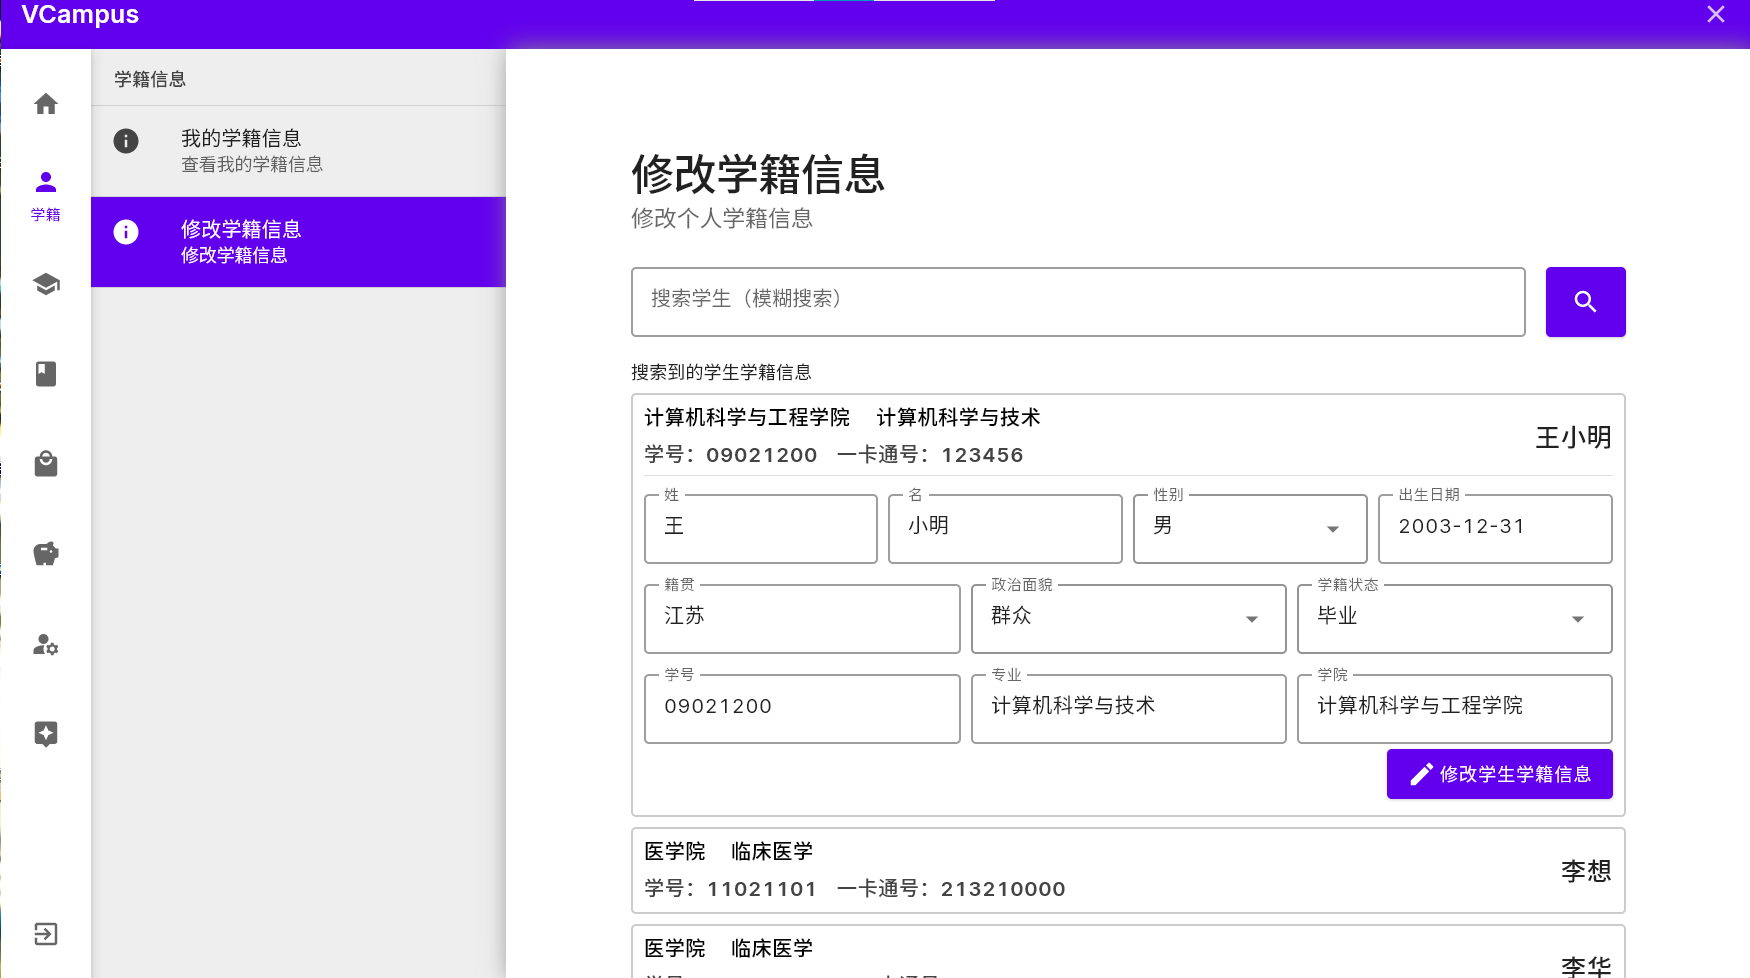
\includegraphics[width=\textwidth]{fig/student_status/student-status-modify.png}}
\textbf{修改学籍界面}
\end{center}

\subsection{教务}

\subsubsection{我的课表}
在我的课表界面,学生可以通过切换周次来获取不同周次的课程。其风格完全按照当前按主流大学生使用的课程表界面布局,简洁、大方,一目了然。该权限给学生开放。
\begin{center}
\shadowbox{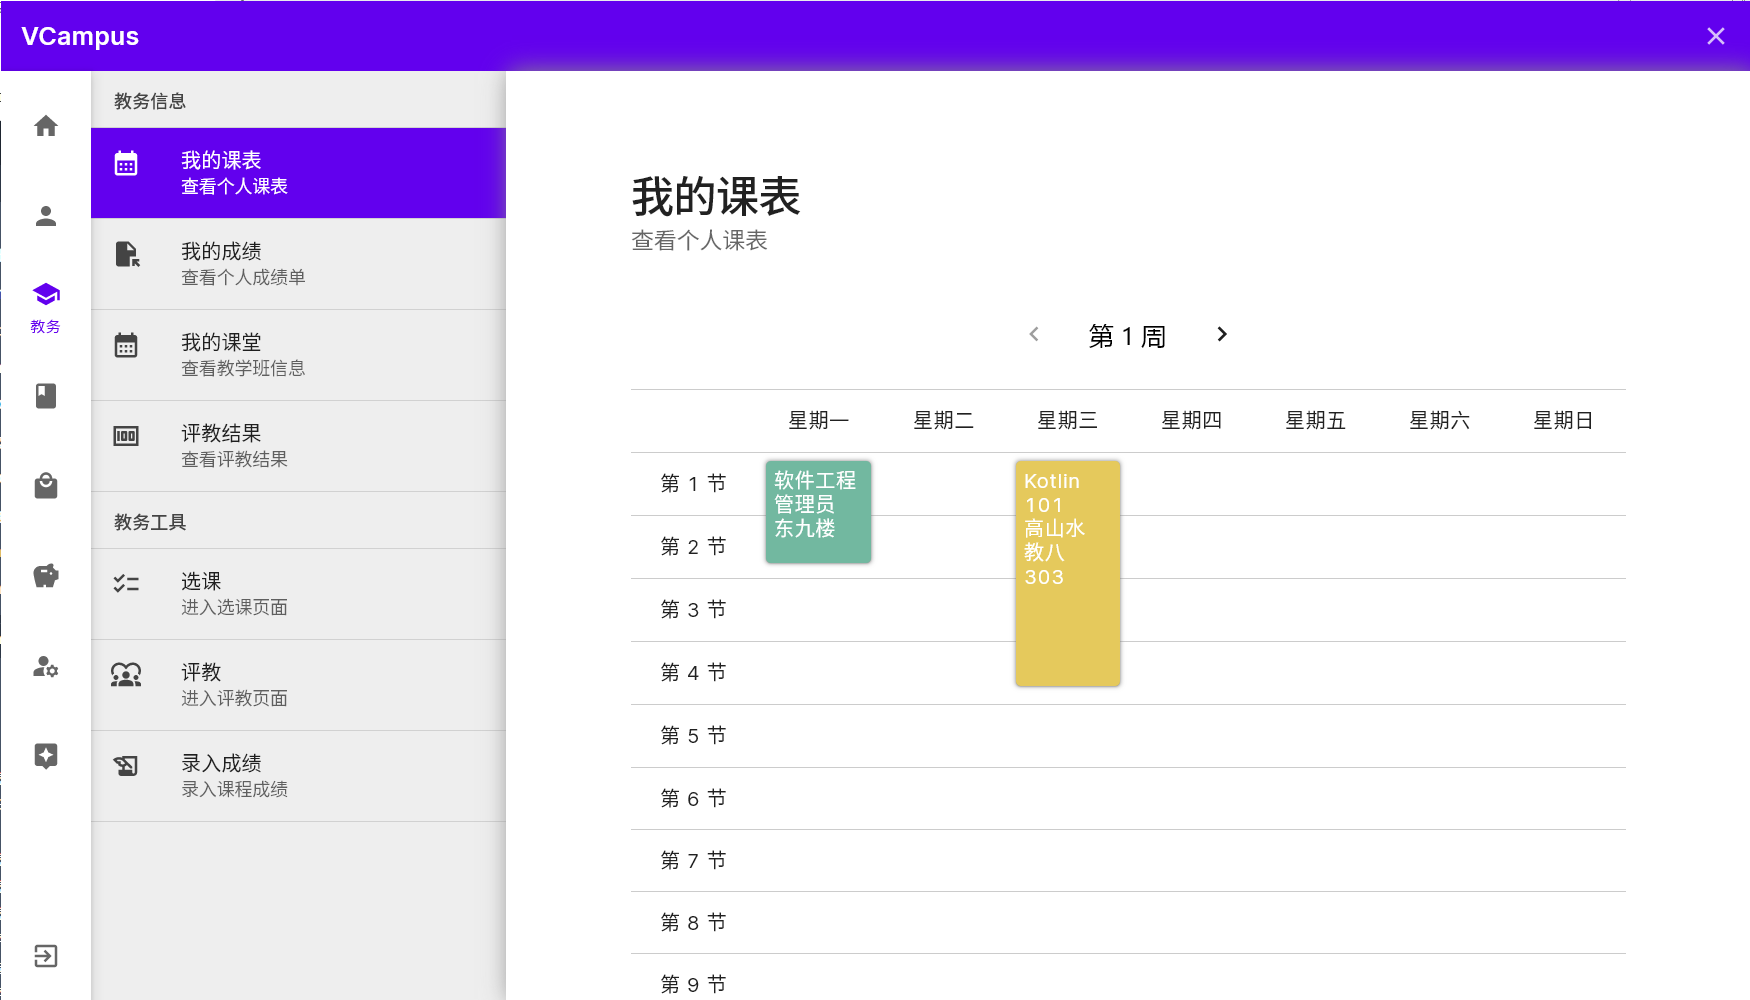
\includegraphics[width=\textwidth]{fig/teaching_affairs/classTable.png}}
\textbf{我的课表界面}
\end{center}

\subsubsection{我的成绩}
学生可以通过我的成绩界面查看各类成绩以及总成绩,通过单击课程栏来展开某门课程的各种成绩,包括班级的最高和最低成绩以及平均分。
\begin{center}
\shadowbox{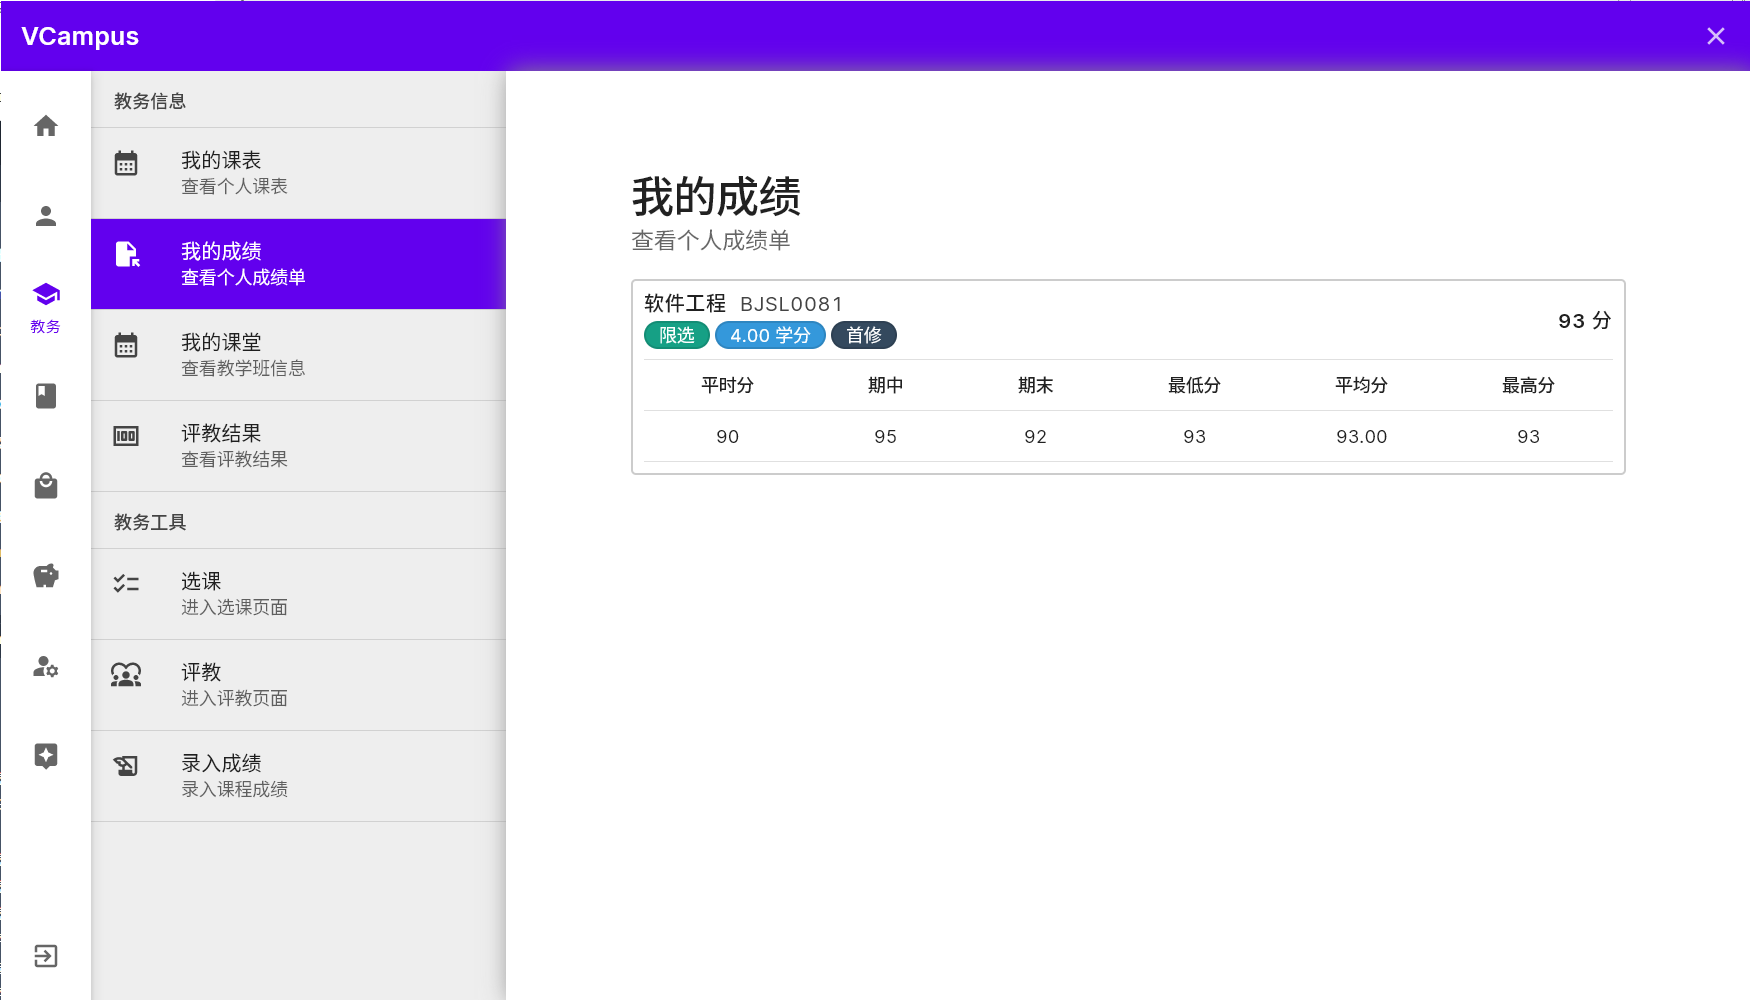
\includegraphics[width=\textwidth]{fig/teaching_affairs/gradeList.png}}
\textbf{我的成绩界面}
\end{center}

\subsubsection{我的课堂}
我的课堂支持通过文件导出的形式将上课学生的名单导出到Excel表格,通过单击学生名单来实现,并支持自由指定文件路径。
\begin{center}
\shadowbox{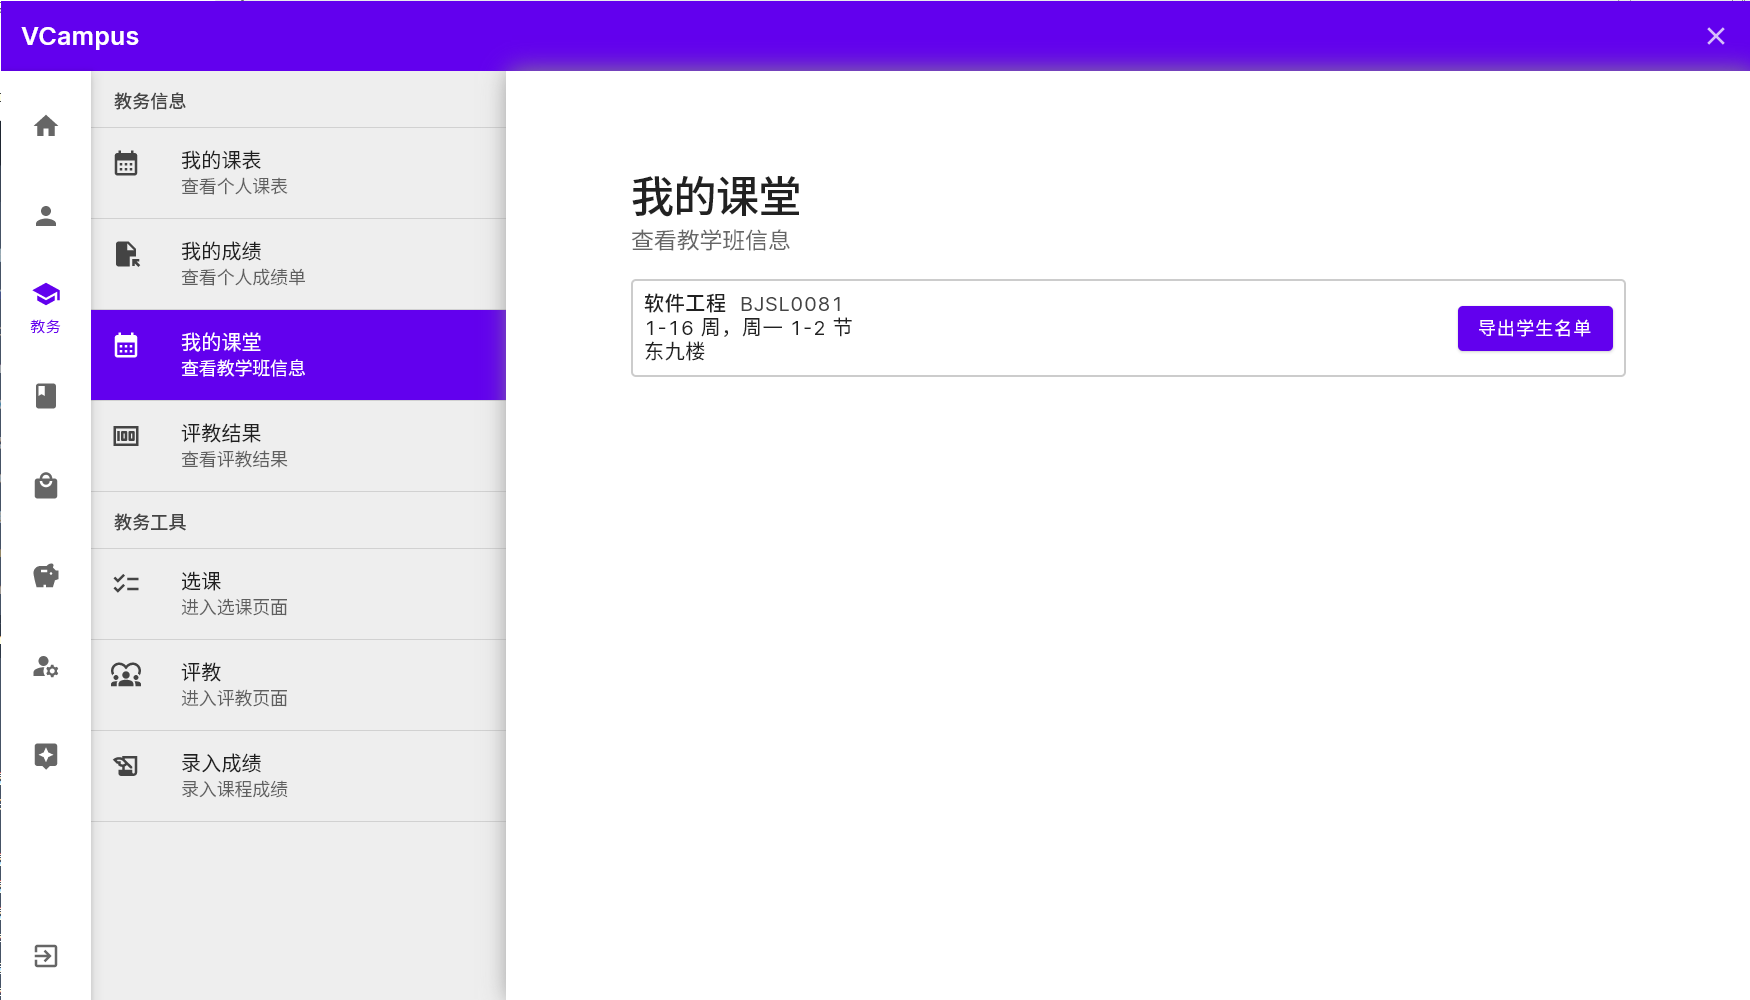
\includegraphics[width=\textwidth]{fig/teaching_affairs/showClass.png}}
\textbf{我的课堂界面}
\end{center}

\subsubsection{评教结果}
评教的课程并列在评教结果消息栏,用户通过单击所要查看的课程来查看评教结果,评教结果包括课堂各方面表现的打分表现和文字评价。
\begin{center}
\shadowbox{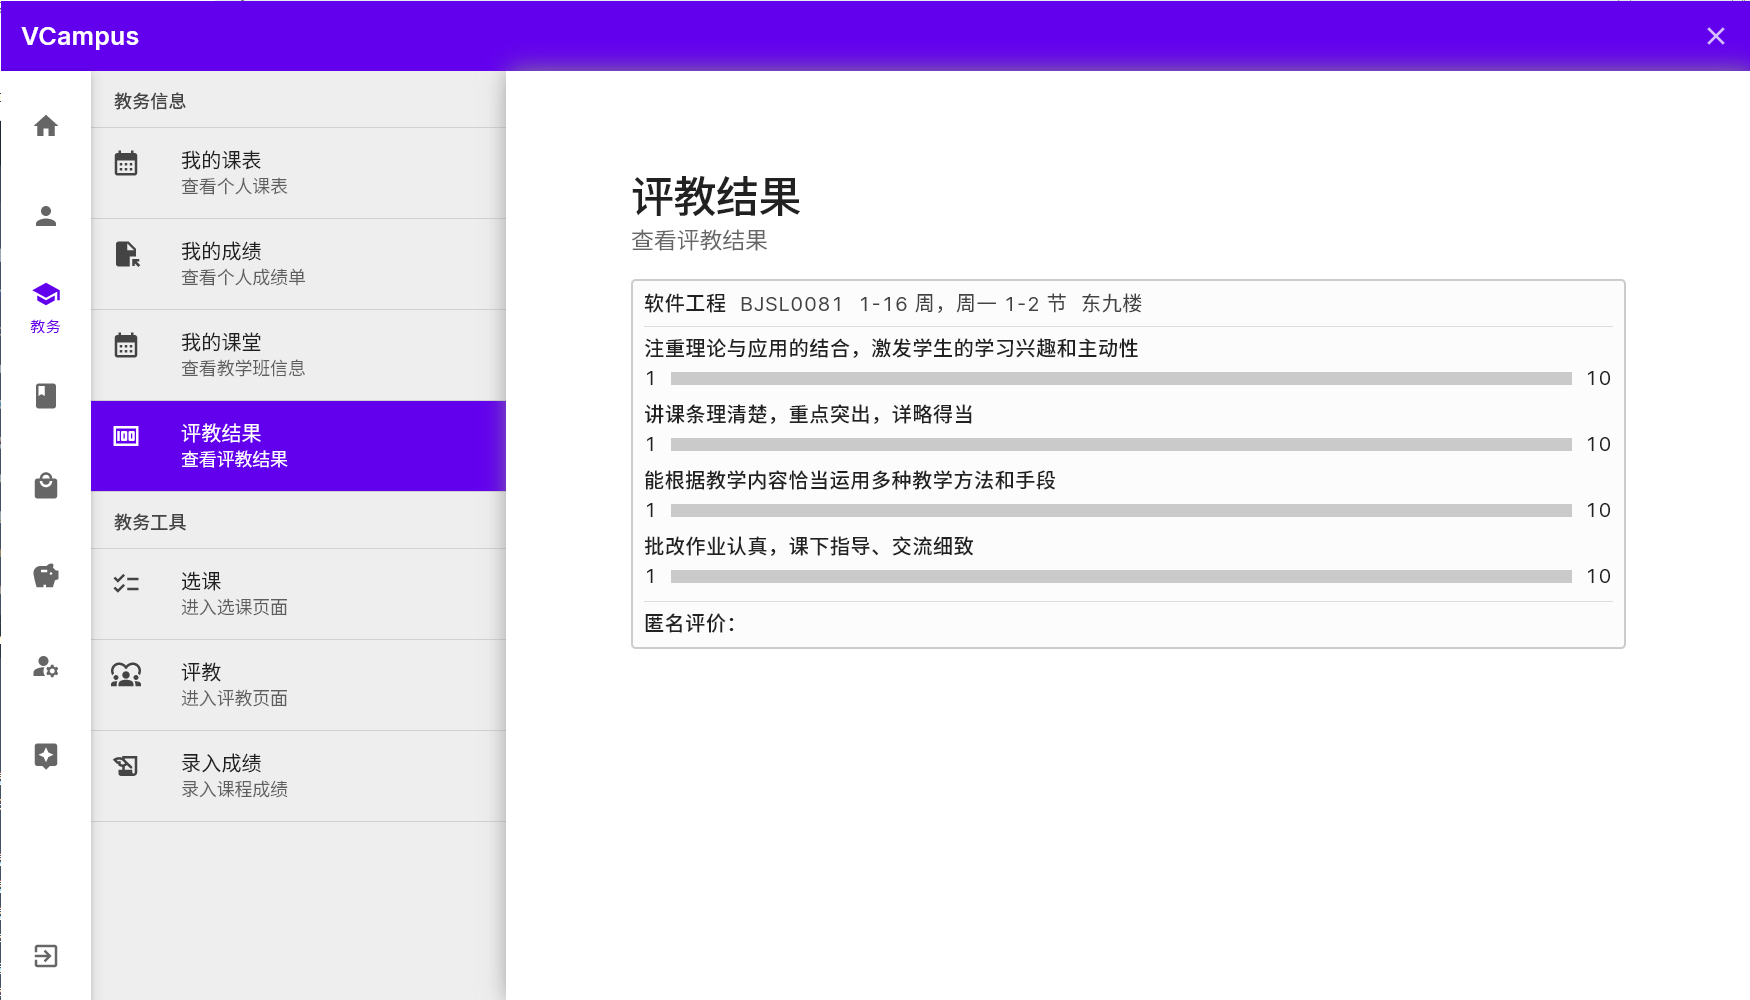
\includegraphics[width=\textwidth]{fig/teaching_affairs/Evaluation-results.png}}
\textbf{评教结果界面}
\end{center}

\subsubsection{选课}
该选课界面参照东南大学使用的选课界面,通过单击课程栏来显示可供选择的教学班,并且可以自由查看任课教师,上课时间和地点以及是否首修等基本信息。如若时间冲突则或课容量已满则不可再选该门课程,并且支持退选。
\begin{center}
\shadowbox{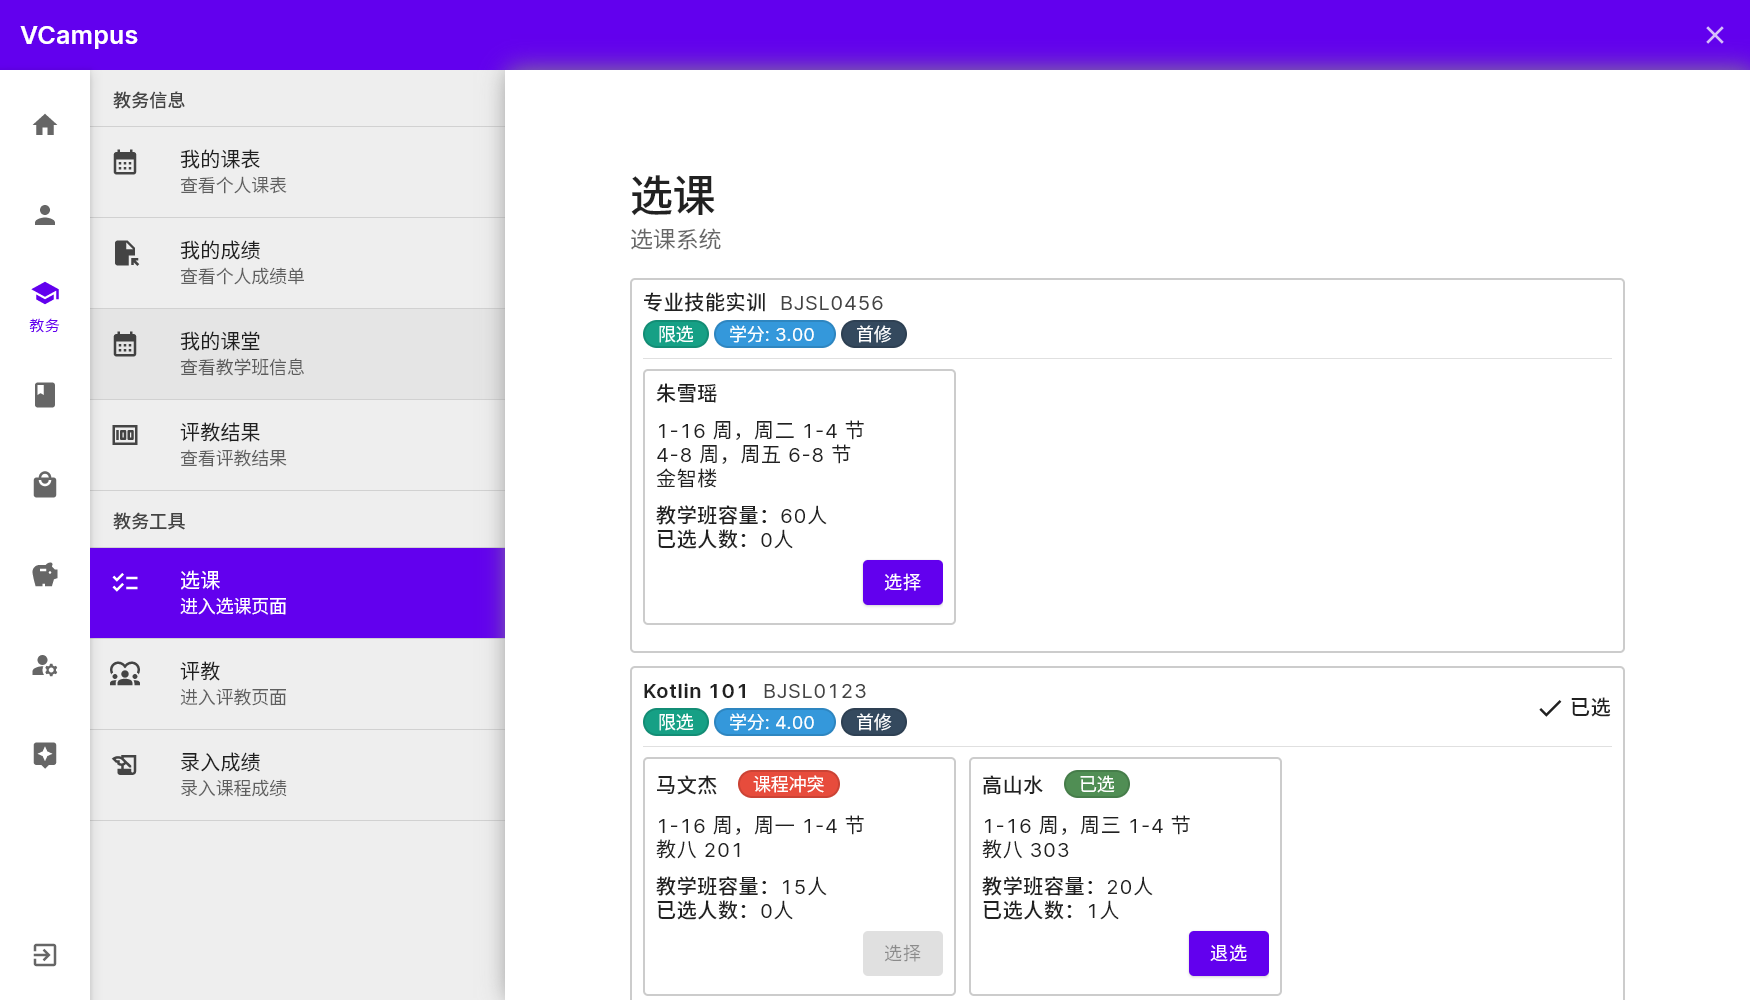
\includegraphics[width=\textwidth]{fig/teaching_affairs/selectClass.png}}
\textbf{选课界面}
\end{center}

\subsubsection{评教}
通过单击课程栏来展开评教信息,评教分为五个方面,支持从教学的不同的方面打分,单击相应的分数项即可完成打分。还支持输入文字评价来更一步完善评教体系,最后通过单击提交进行提交。
\begin{center}
\shadowbox{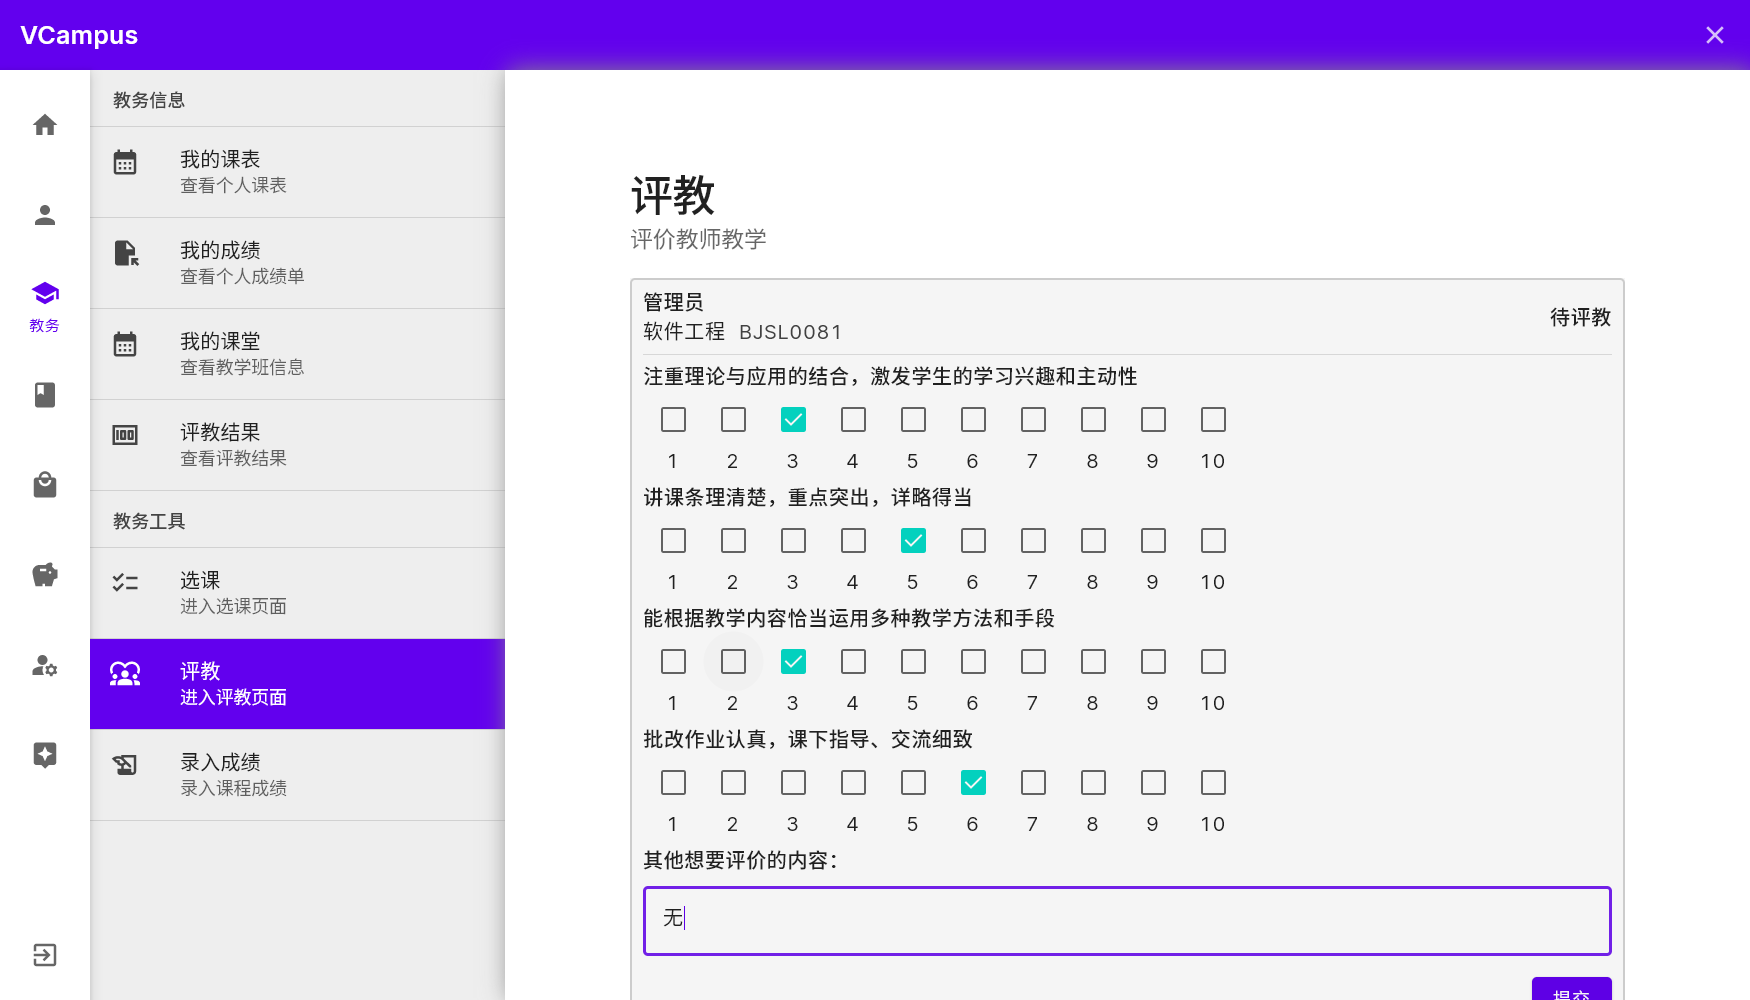
\includegraphics[width=\textwidth]{fig/teaching_affairs/Evaluate.png}}
\textbf{评教界面}
\end{center}

\subsubsection{录入成绩}
录入成绩功能支持从Excel表格导入和导出成绩,只需将要录入的成绩输入到Excel表格并导入即可。不同于传统的录入方式,Excel录入可以更加方便的进行批量操作,例如计算总成绩等。
\begin{center}
\shadowbox{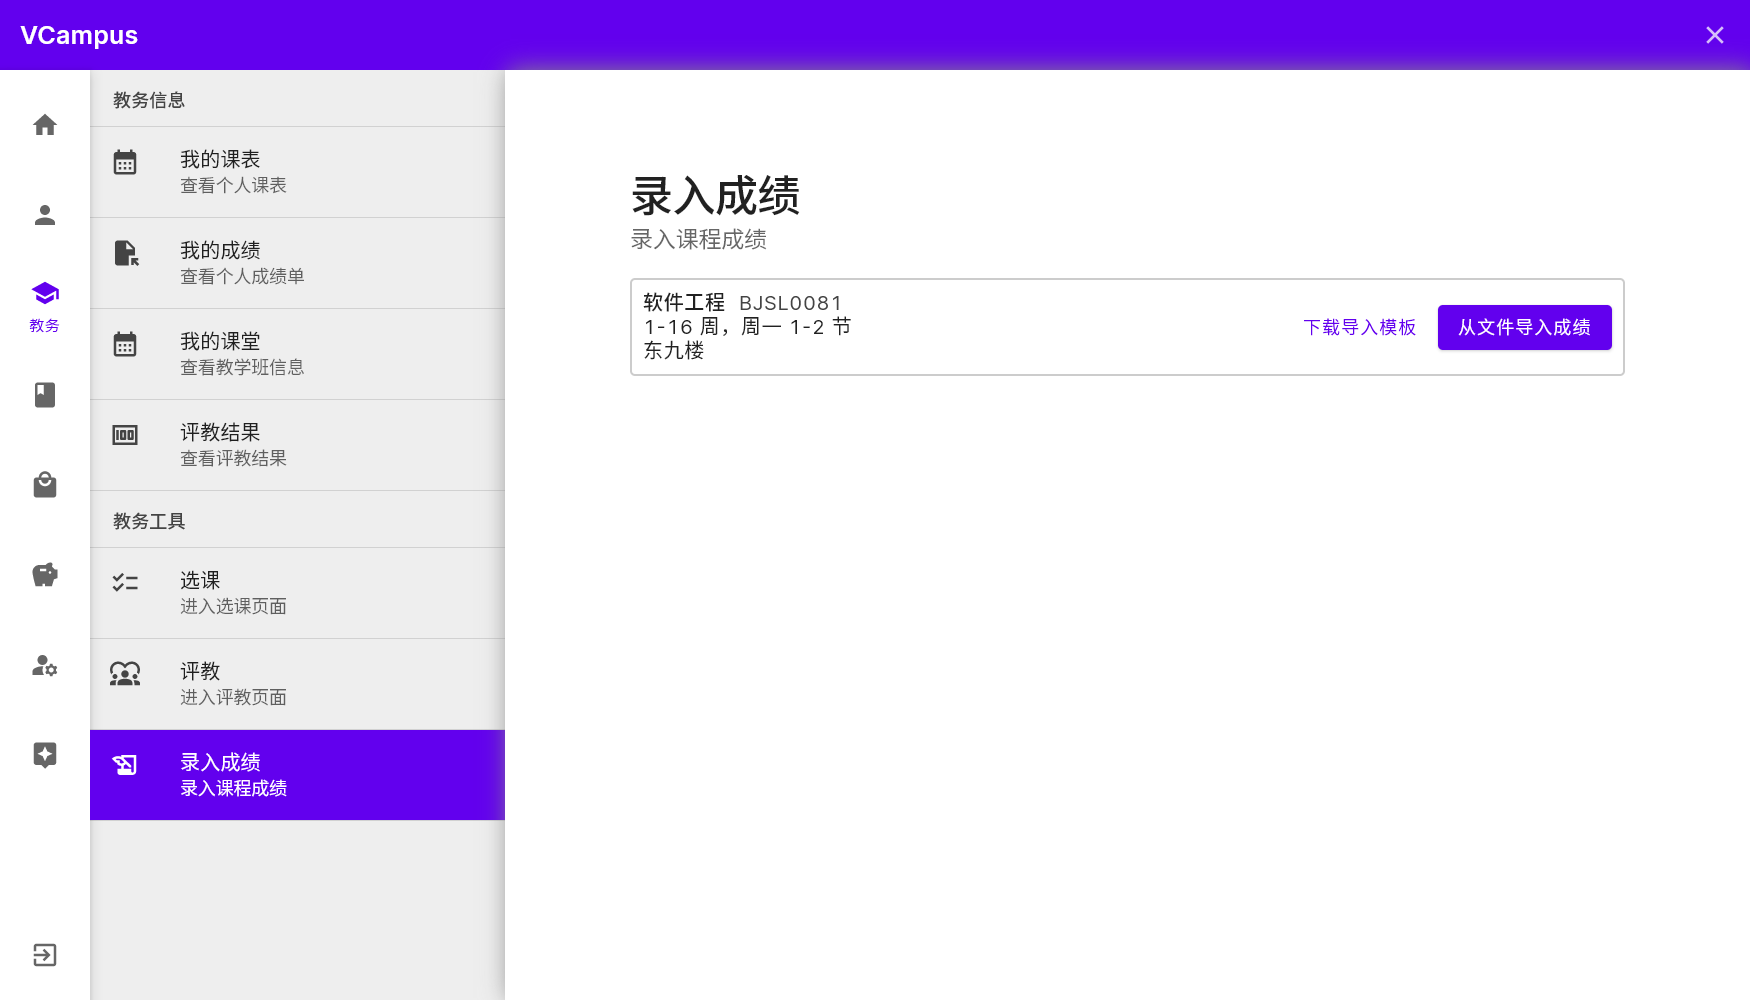
\includegraphics[width=\textwidth]{fig/teaching_affairs/Entry-results.png}}
\textbf{录入成绩界面}
\end{center}


\subsection{图书馆}

\subsubsection{查询图书}
用户可通过输入关键词对图书进行检索(支持模糊检索),界面会返回与关键词相关的图书列表,显示书名、作者、出版社以及馆藏副本、可借副本等基础信息,当点击图书时会展开图书的具体信息,包括图书ISBN、简介、书籍状态、馆藏地等详细信息,查询图书界面如下所示:

\begin{center}
\shadowbox{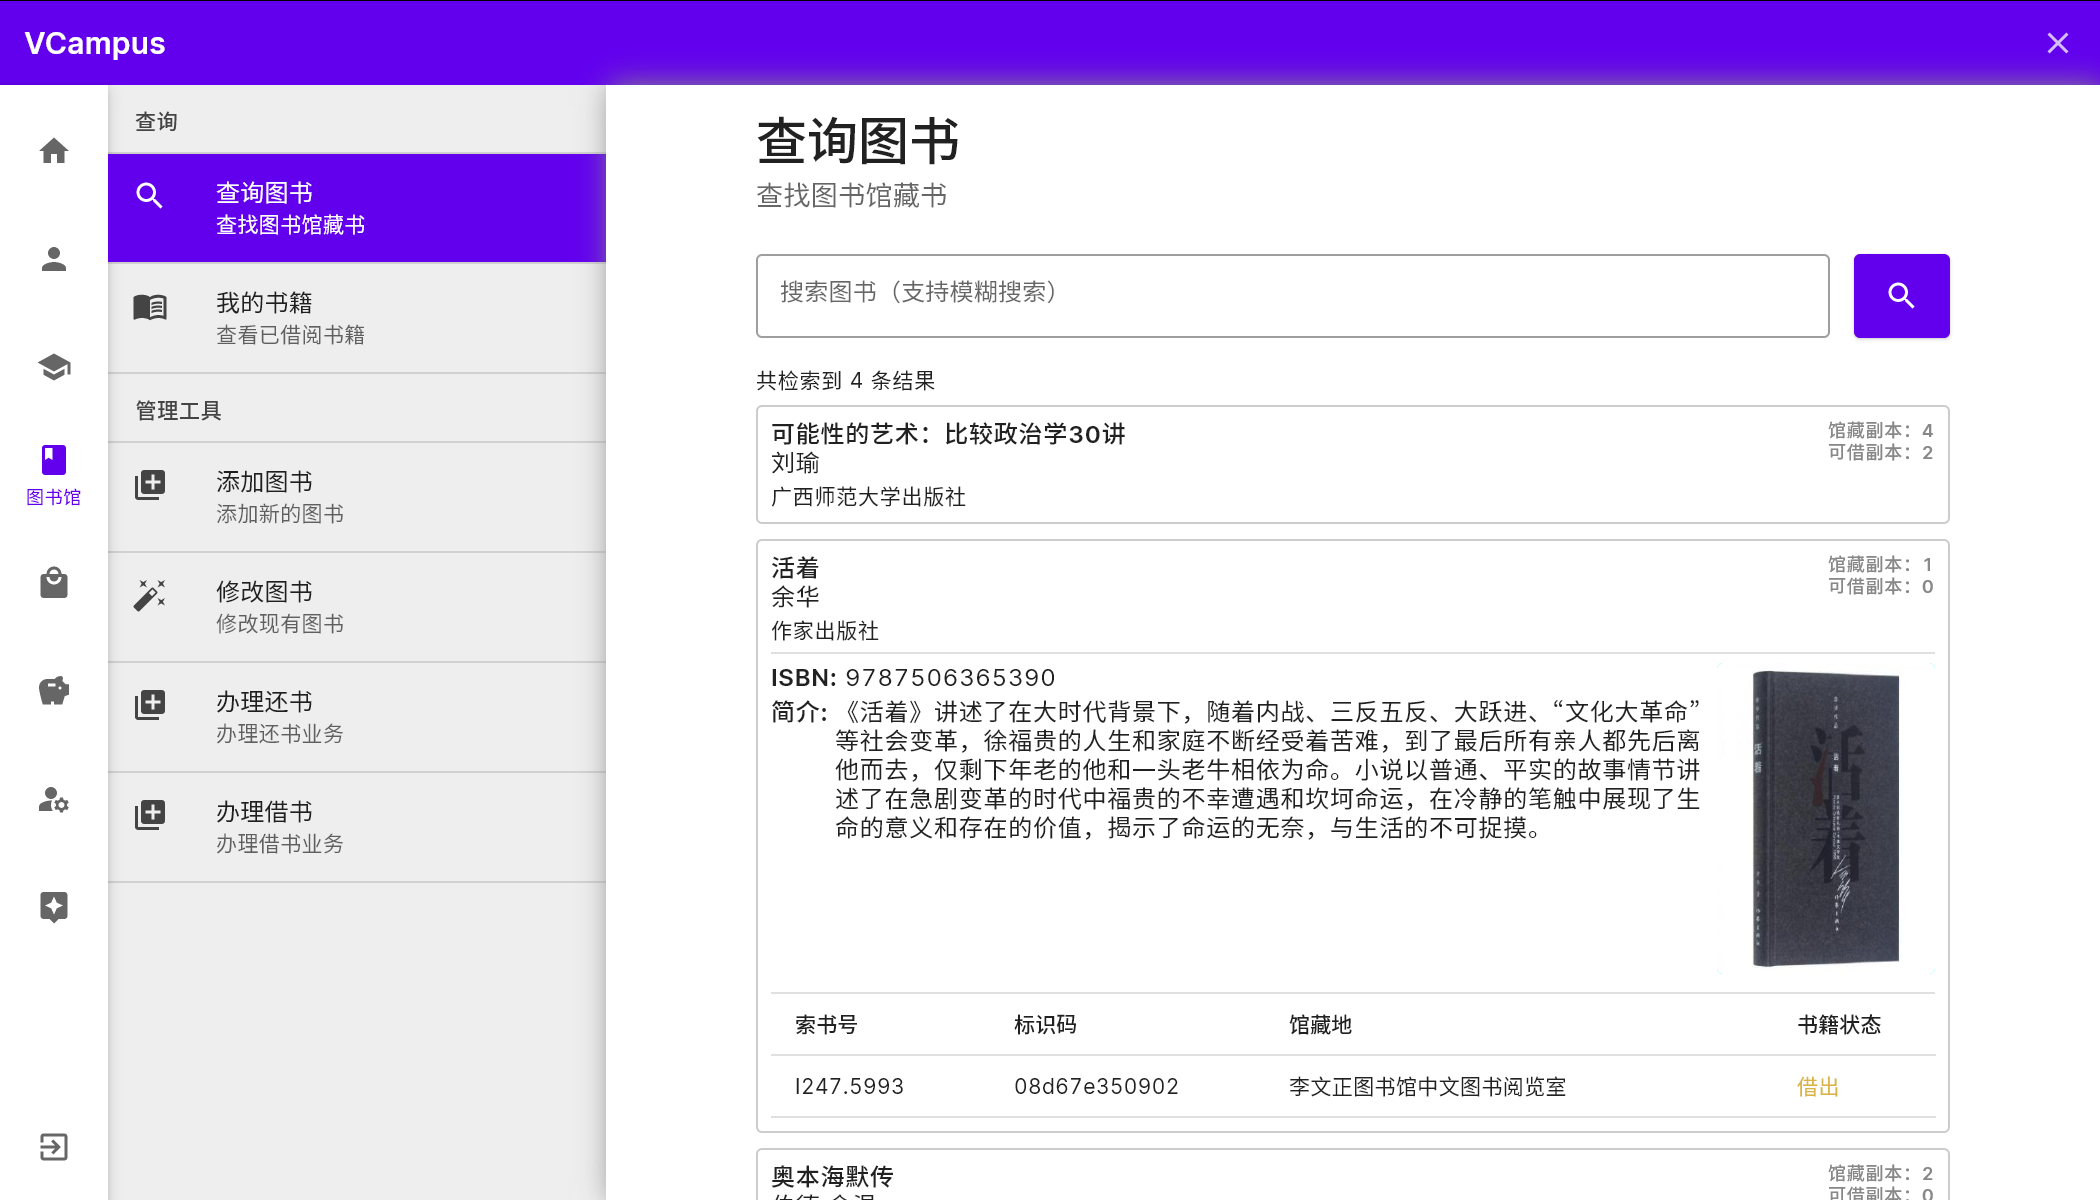
\includegraphics[width=\textwidth]{fig/library/search_book.png}}
\textbf{查询图书界面}
\end{center}


\subsubsection{我的书籍}
我的书籍界面会显示用户已借书籍,向用户展示借书时间和应还时间等,用户可点击续借,然后图书应还日期会延后一个月,具体页面设计如下所示:

\begin{center}
\shadowbox{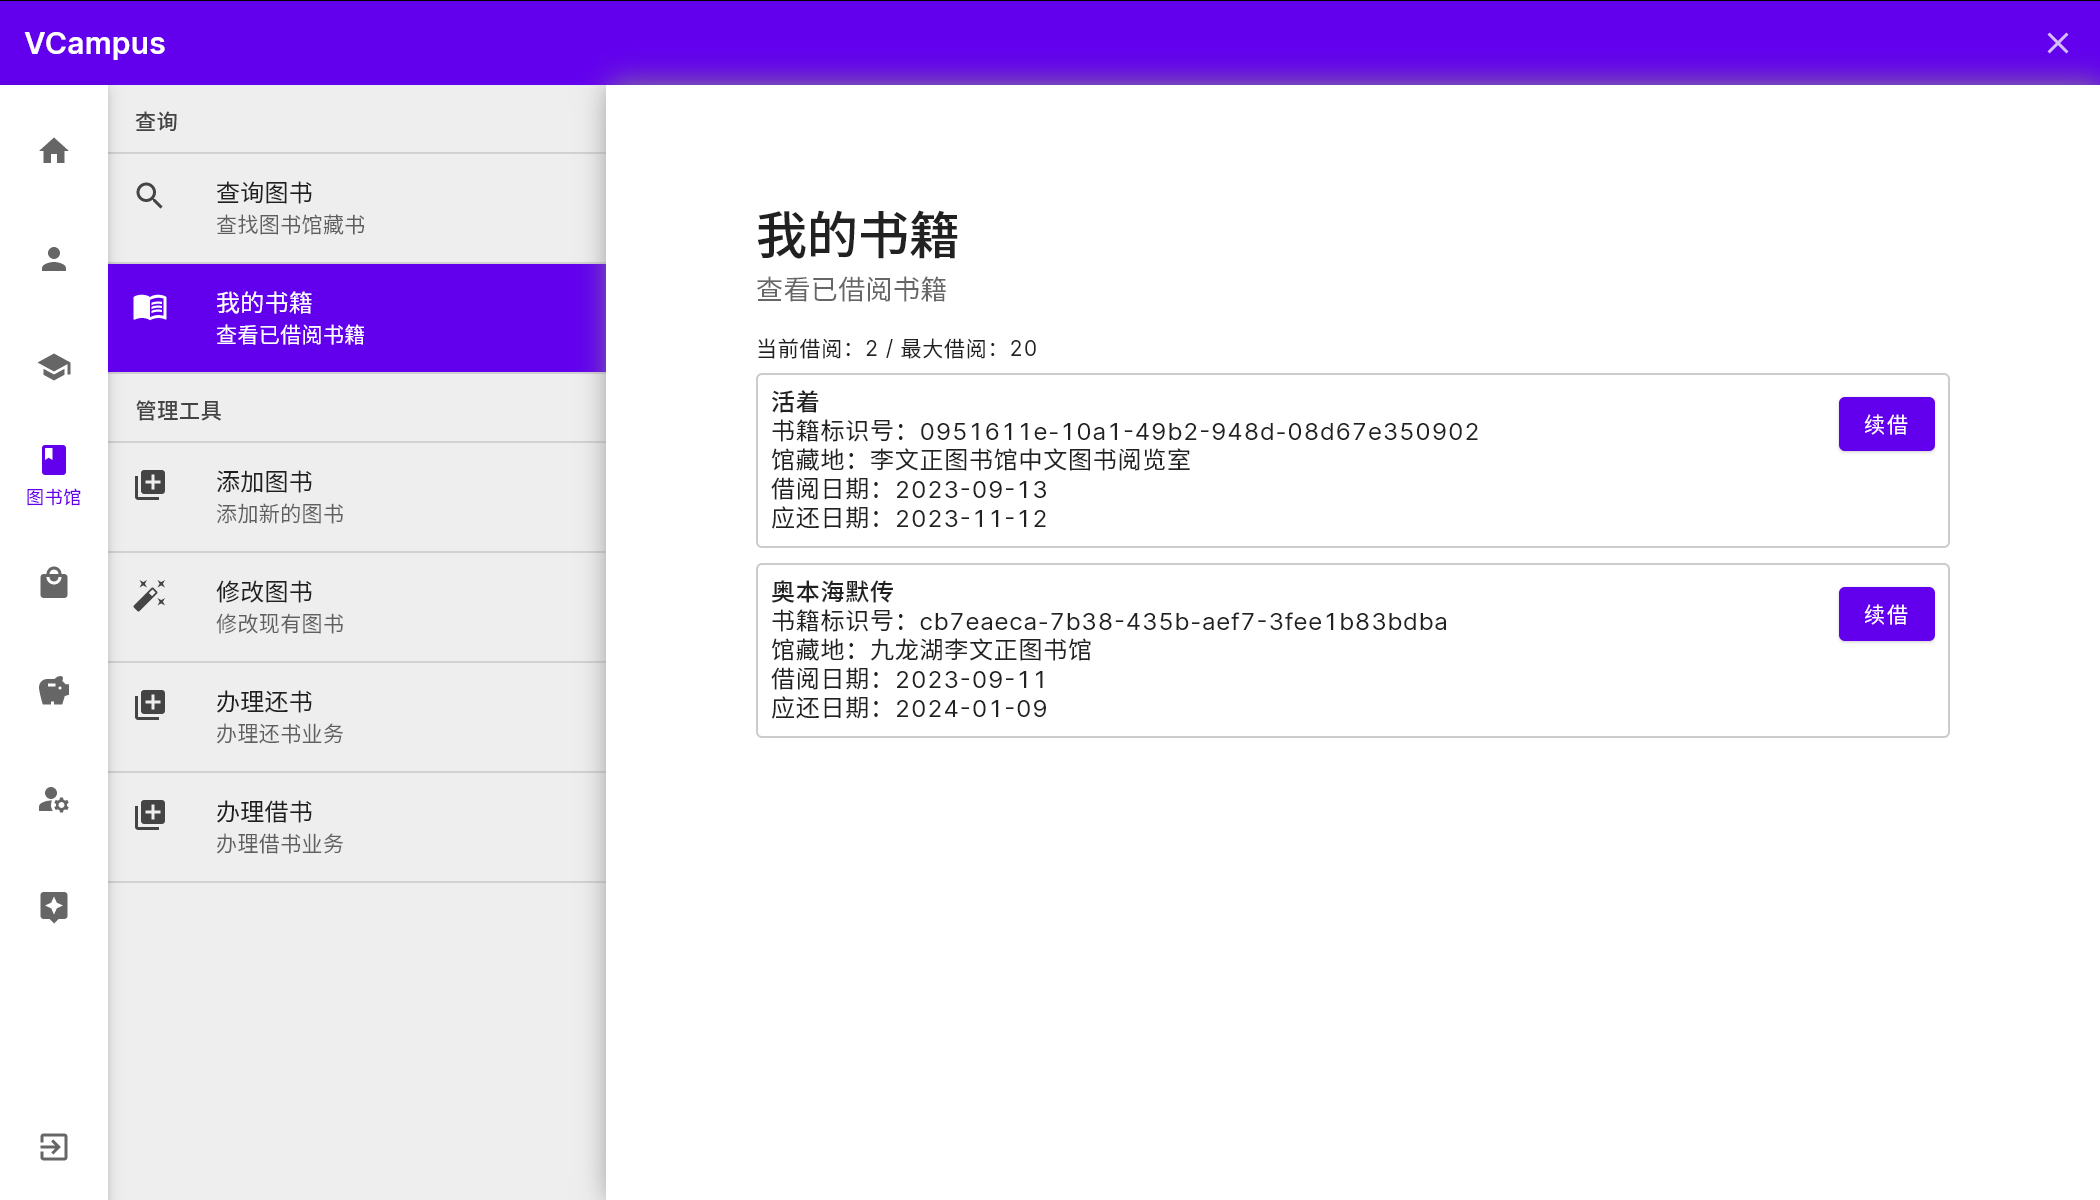
\includegraphics[width=\textwidth]{fig/library/my_book.png}}
\textbf{我的书籍界面}
\end{center}


\subsubsection{添加图书}
此页面是为管理员新增图书而设计的,管理员可以通过输入图书ISBN编号一键获取图书信息,然后手动添加图书简介、索书号等信息.

\begin{center}
\shadowbox{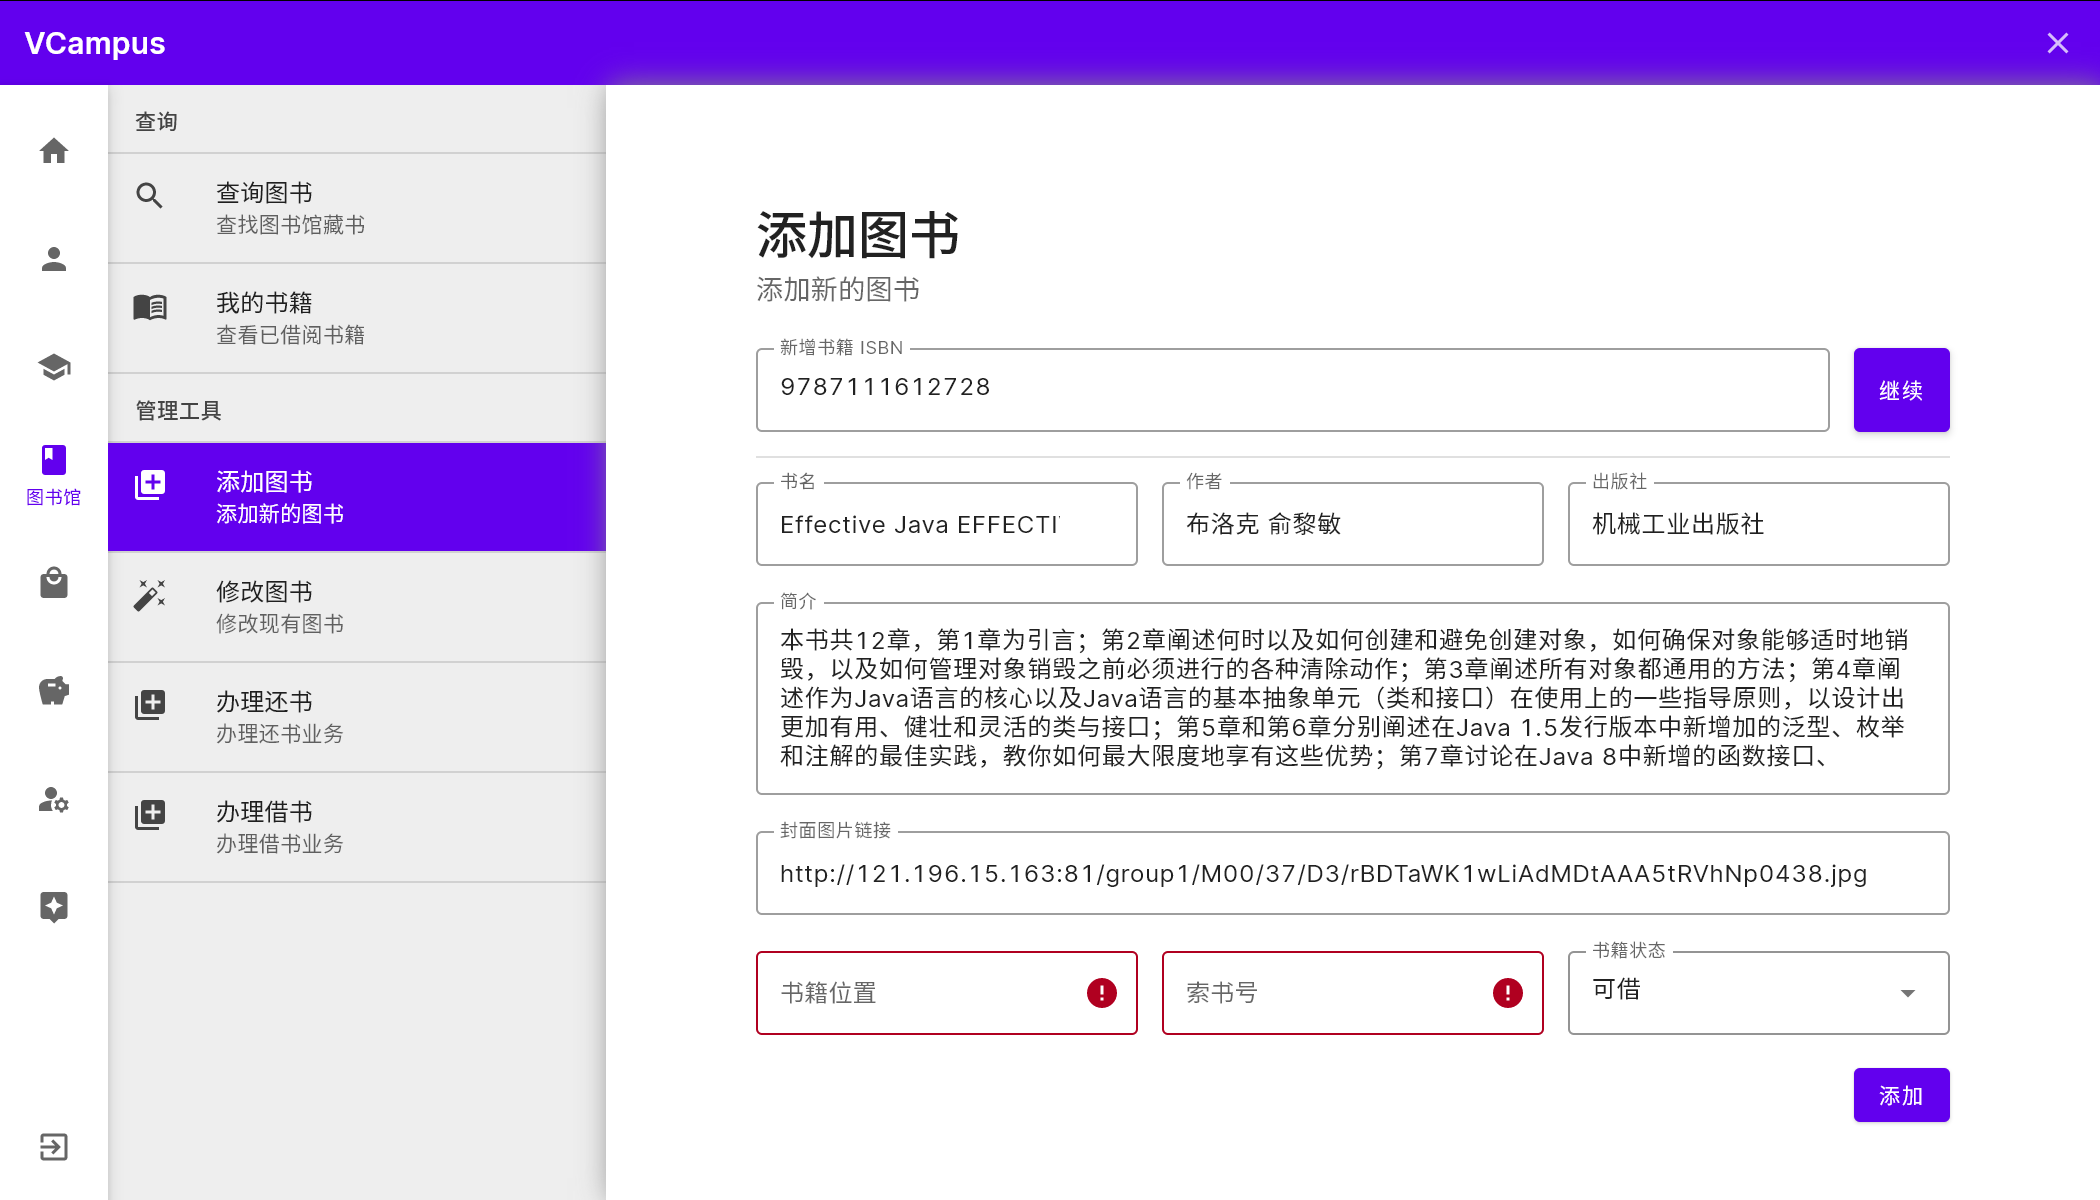
\includegraphics[width=\textwidth]{fig/library/add_book.png}}
\textbf{添加图书界面}
\end{center}

\subsubsection{修改图书}
管理员可在修改图书界面首先通过关键词查询图书,点击图书展开后可以通过点击“修改图书信息"按钮来对图书进行修改,包括修改索书号、馆藏地、书籍状态等,还可以在此界面进行删除图书副本的操作.

\begin{center}
\shadowbox{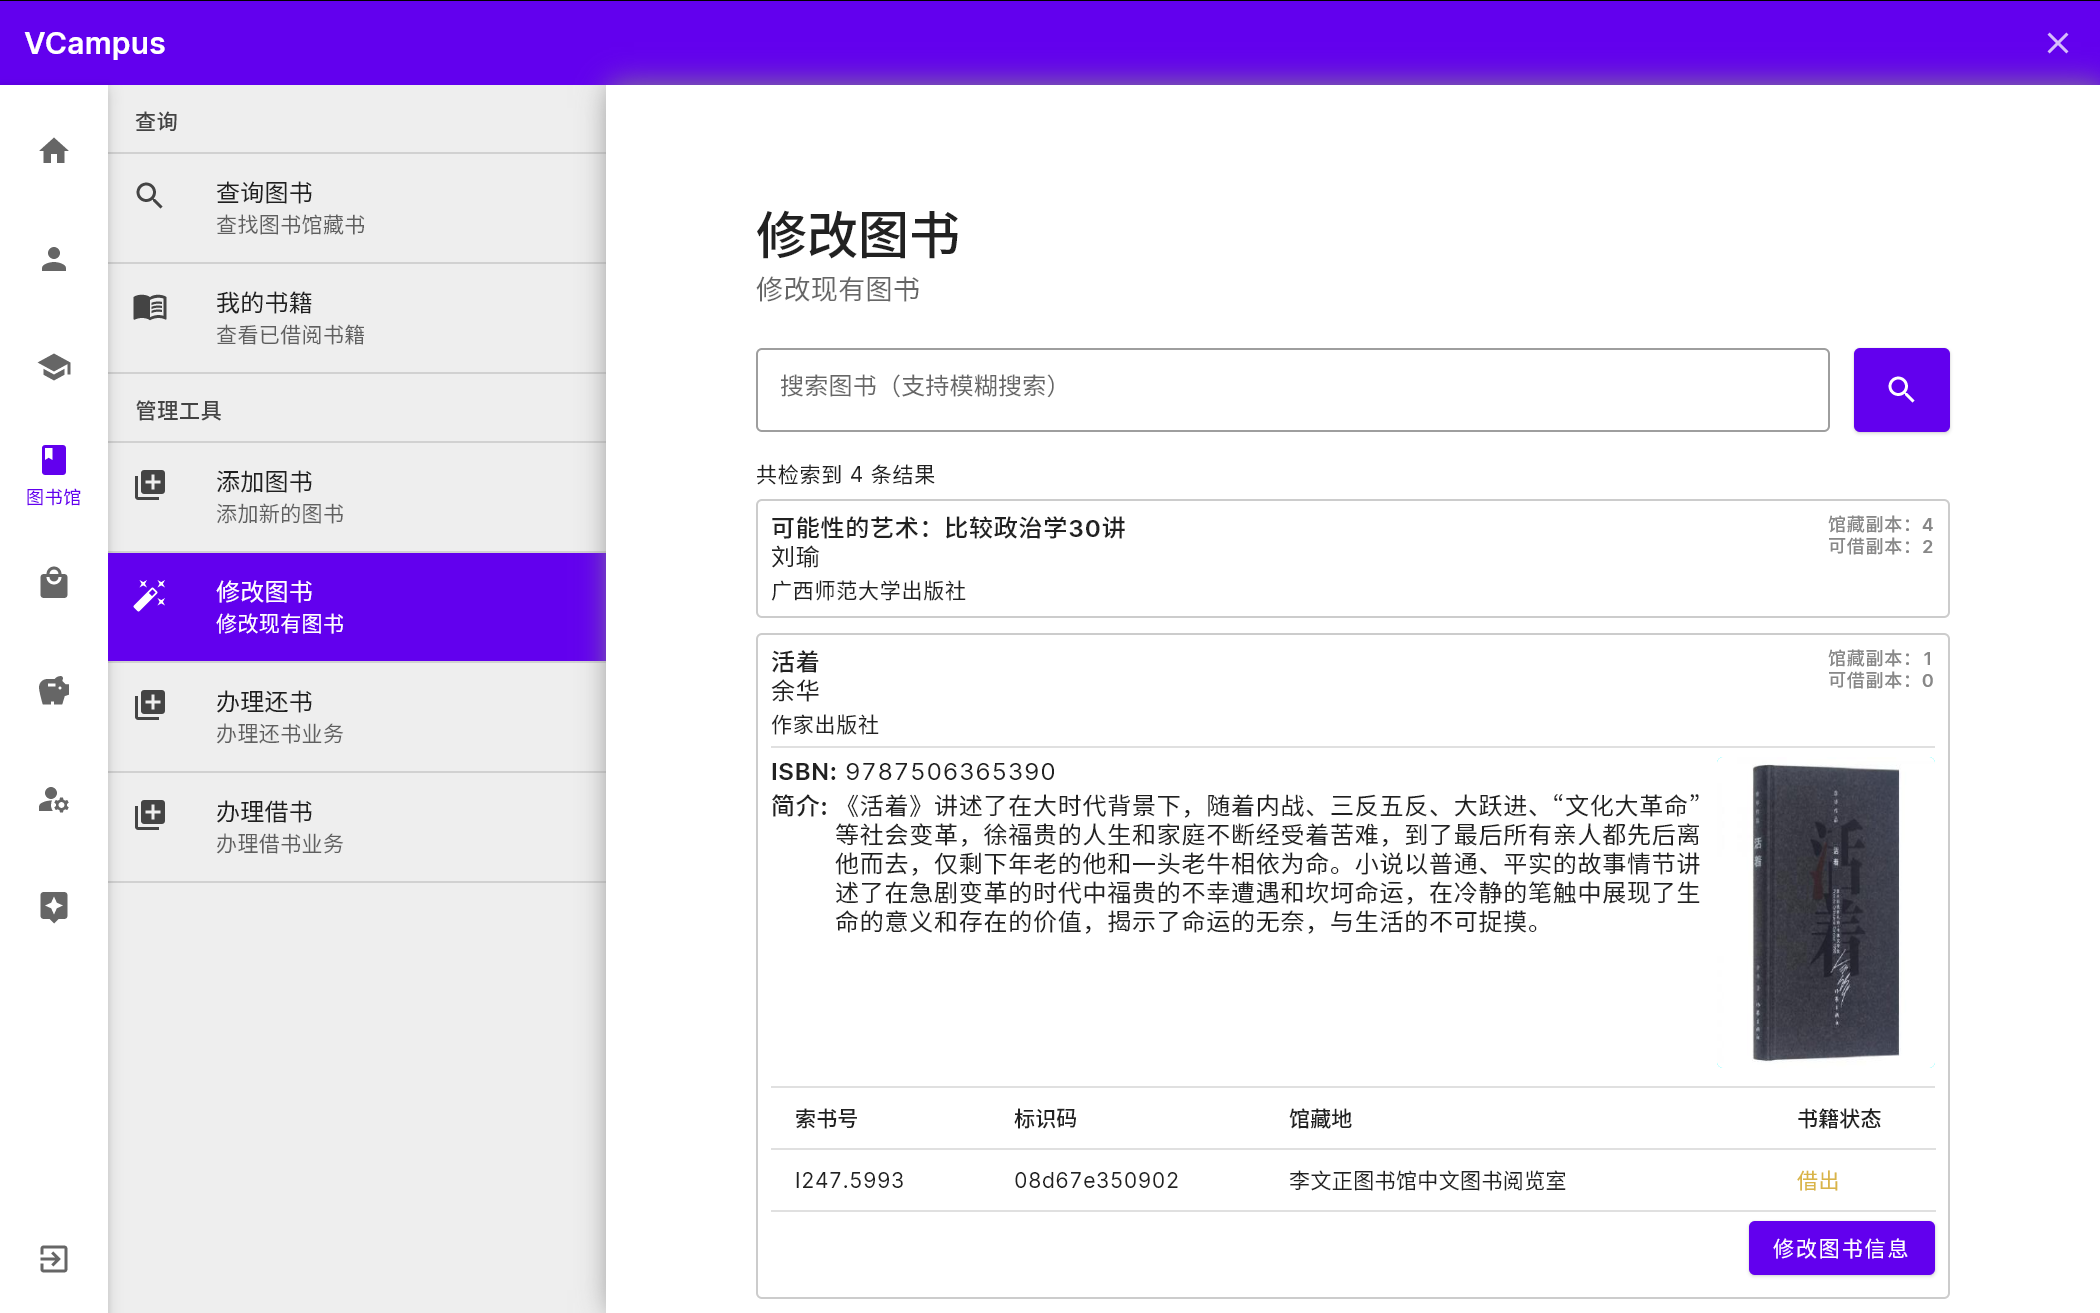
\includegraphics[width=\textwidth]{fig/library/modify_book.png}}
\textbf{修改图书界面}
\end{center}

\subsubsection{办理还书}
管理员可在此处登记用户还书、为用户办理续借,通过点击搜索图标或者按下enter键可搜索用户一卡通号以展示其借阅状况,通过点击“续借”与“还书”为用户办理对应业务.

\begin{center}
\shadowbox{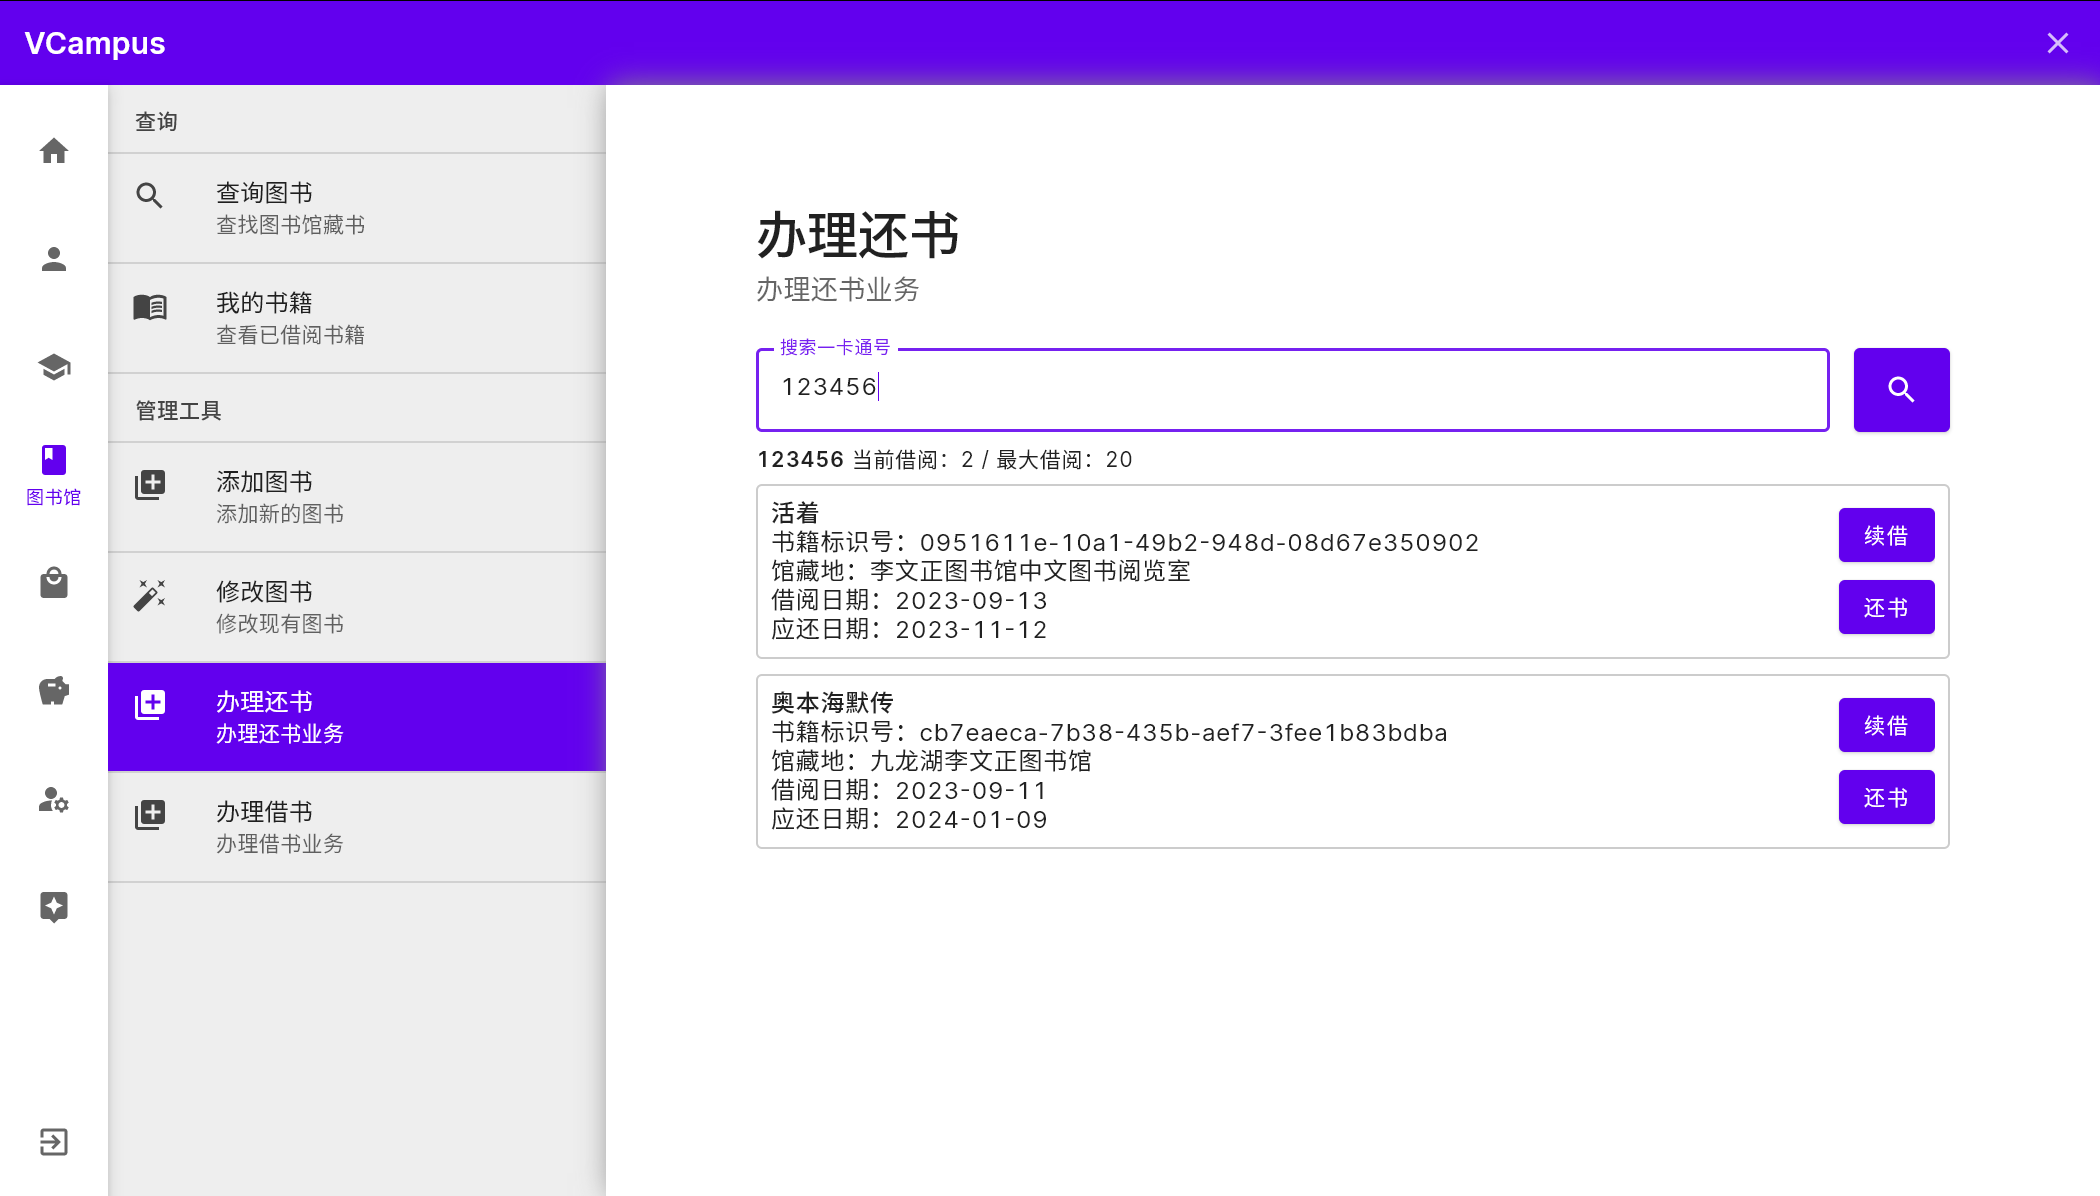
\includegraphics[width=\textwidth]{fig/library/return_book.png}}
\textbf{办理还书界面}
\end{center}

\subsubsection{办理借书}
管理员可在此登记用户借书,通过输入用户一卡通号与书籍UUID(示例一卡通号:123456;示例UUID:98b209af-8e8d-4245-9339-e74c74756469
),可以为用户办理借书,当按下enter键或点击借阅按钮,会登记用户借书,并在屏幕下方显示相应提示(借阅成功或借阅失败).

\begin{center}
\shadowbox{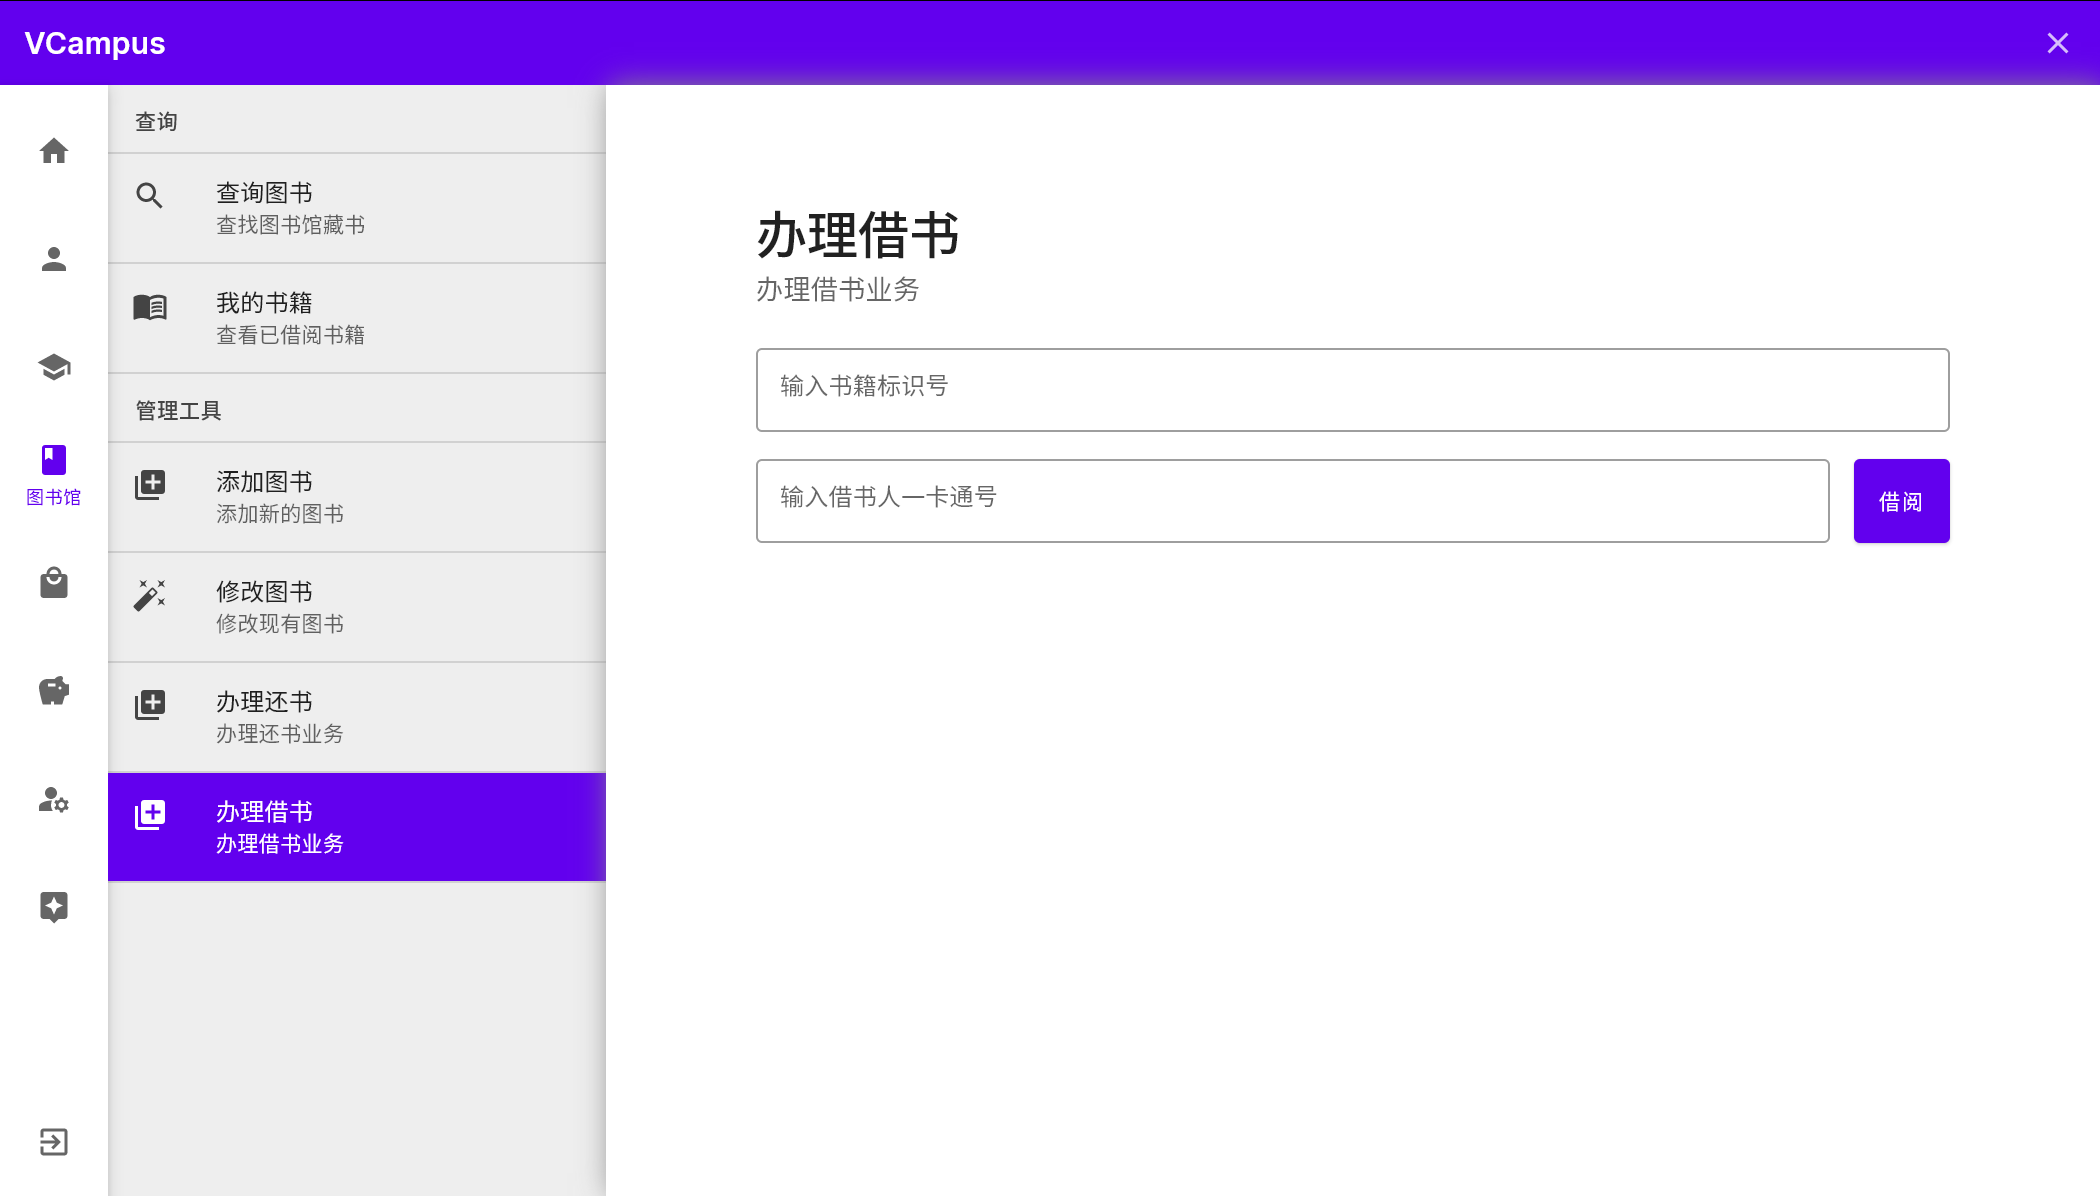
\includegraphics[width=\textwidth]{fig/library/borrow_book.png}}
\textbf{办理借书界面}
\end{center}


\subsection{超市}


\subsubsection{购物页面}

购物页面展示了所有的商品,每个商品都显示了图片、名称和价格。用户可以通过点击每个商品框右下角的加号来将一定数量的商品添加至购物车。除了浏览商品,还可以在上方的搜索框输入关键词,直接搜索商品,搜索方式支持模糊搜索,可以通过名称、描述、价格等信息中的关键词搜索到对应的商品。\\
选择好商品后,点击最下方的“上滑以计算”进入结算页面。

\begin{center}
\shadowbox{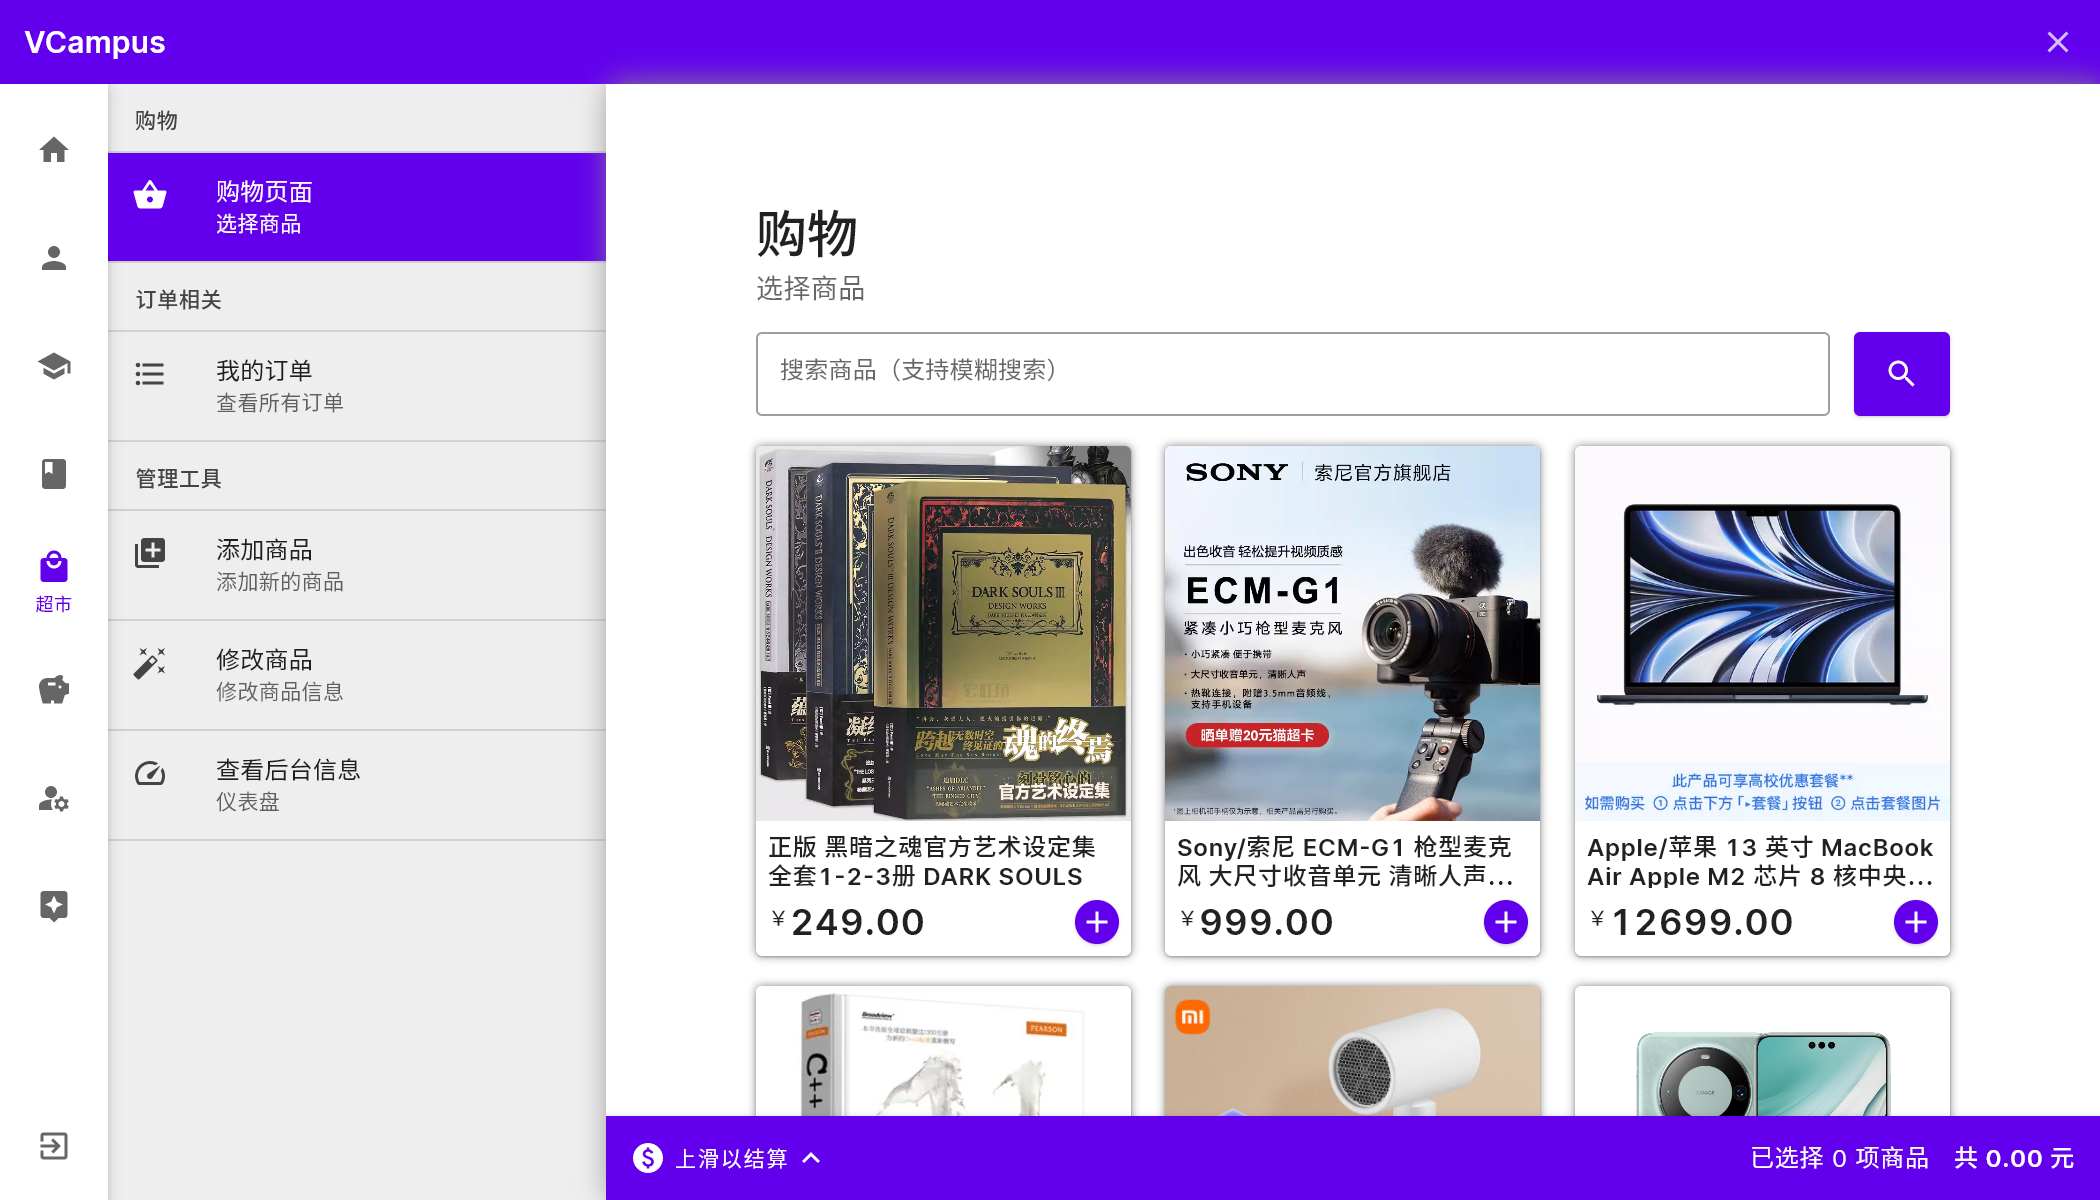
\includegraphics[width=\textwidth]{fig/shop/select_item.png}}
\textbf{购物页面界面}
\end{center}

\subsubsection{我的订单}

订单界面展示了用户的购物信息。所有购物信息按照日期分类,同一天内的消费记录在一起展示。每条消费记录包括商品的图片、名称、价格和个数,最后一天内的消费总金额会展示在下方。用户可以通过“我的订单”界面来查看自己的历史消费记录。

\begin{center}
\shadowbox{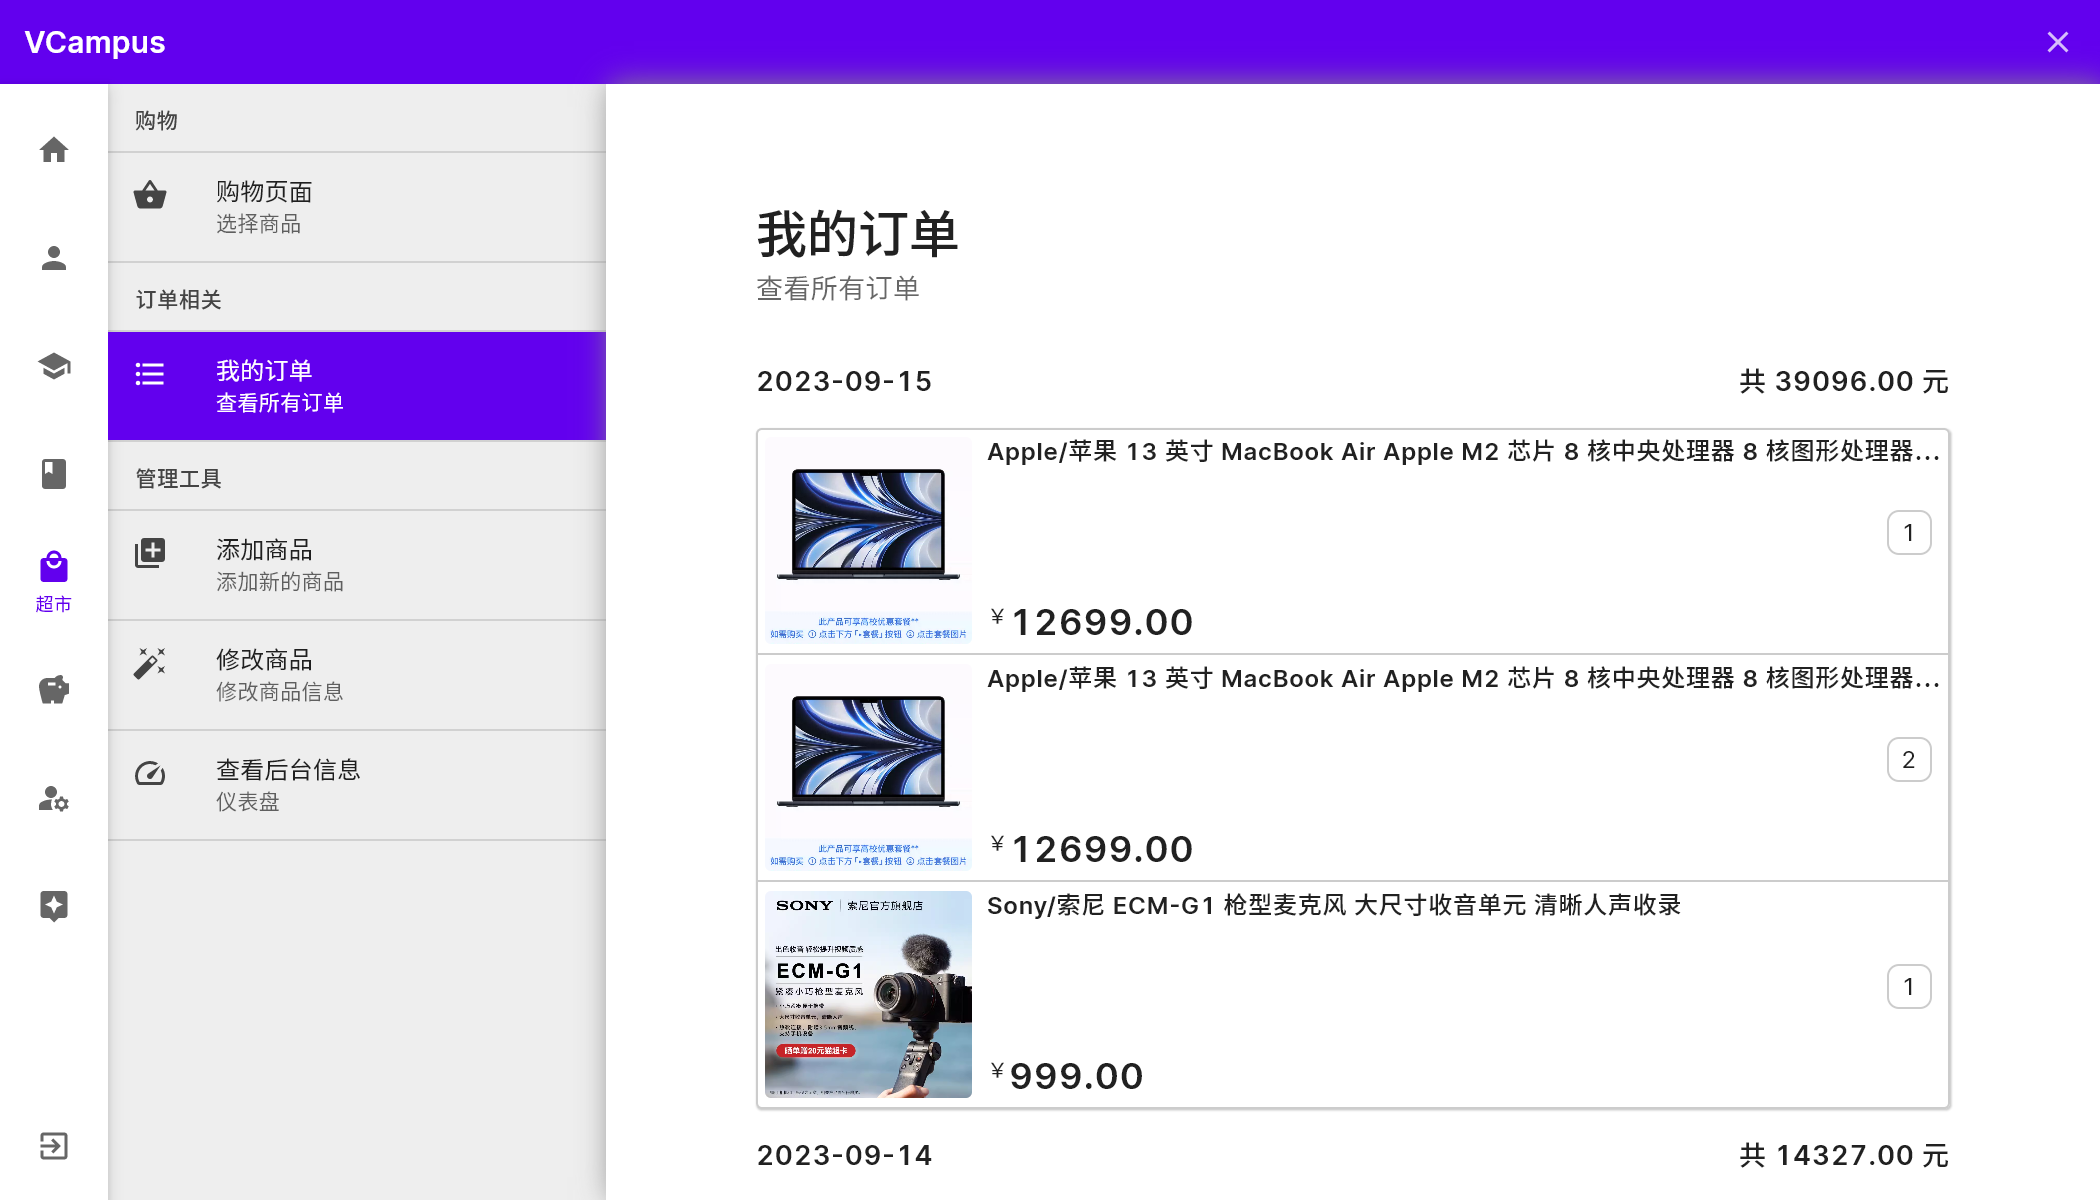
\includegraphics[width=\textwidth]{fig/shop/my_order.png}}
\textbf{我的订单界面}
\end{center}

\subsubsection{添加商品}

添加商品界面是商店管理员的管理界面。管理员在对应的位置填写商品的名称、价格、库存数量,并设置商品的条形码、图片链接和商品介绍。核对信息无误后,点击右下方的“添加商品”提交所有信息,商品就可以创建成功并展示在购物页面。\\
在添加商品信息时要注意信息的合法性,如不能添加已有的商品,商品的条形码为13位,图片链接应为有效链接等。

\begin{center}
\shadowbox{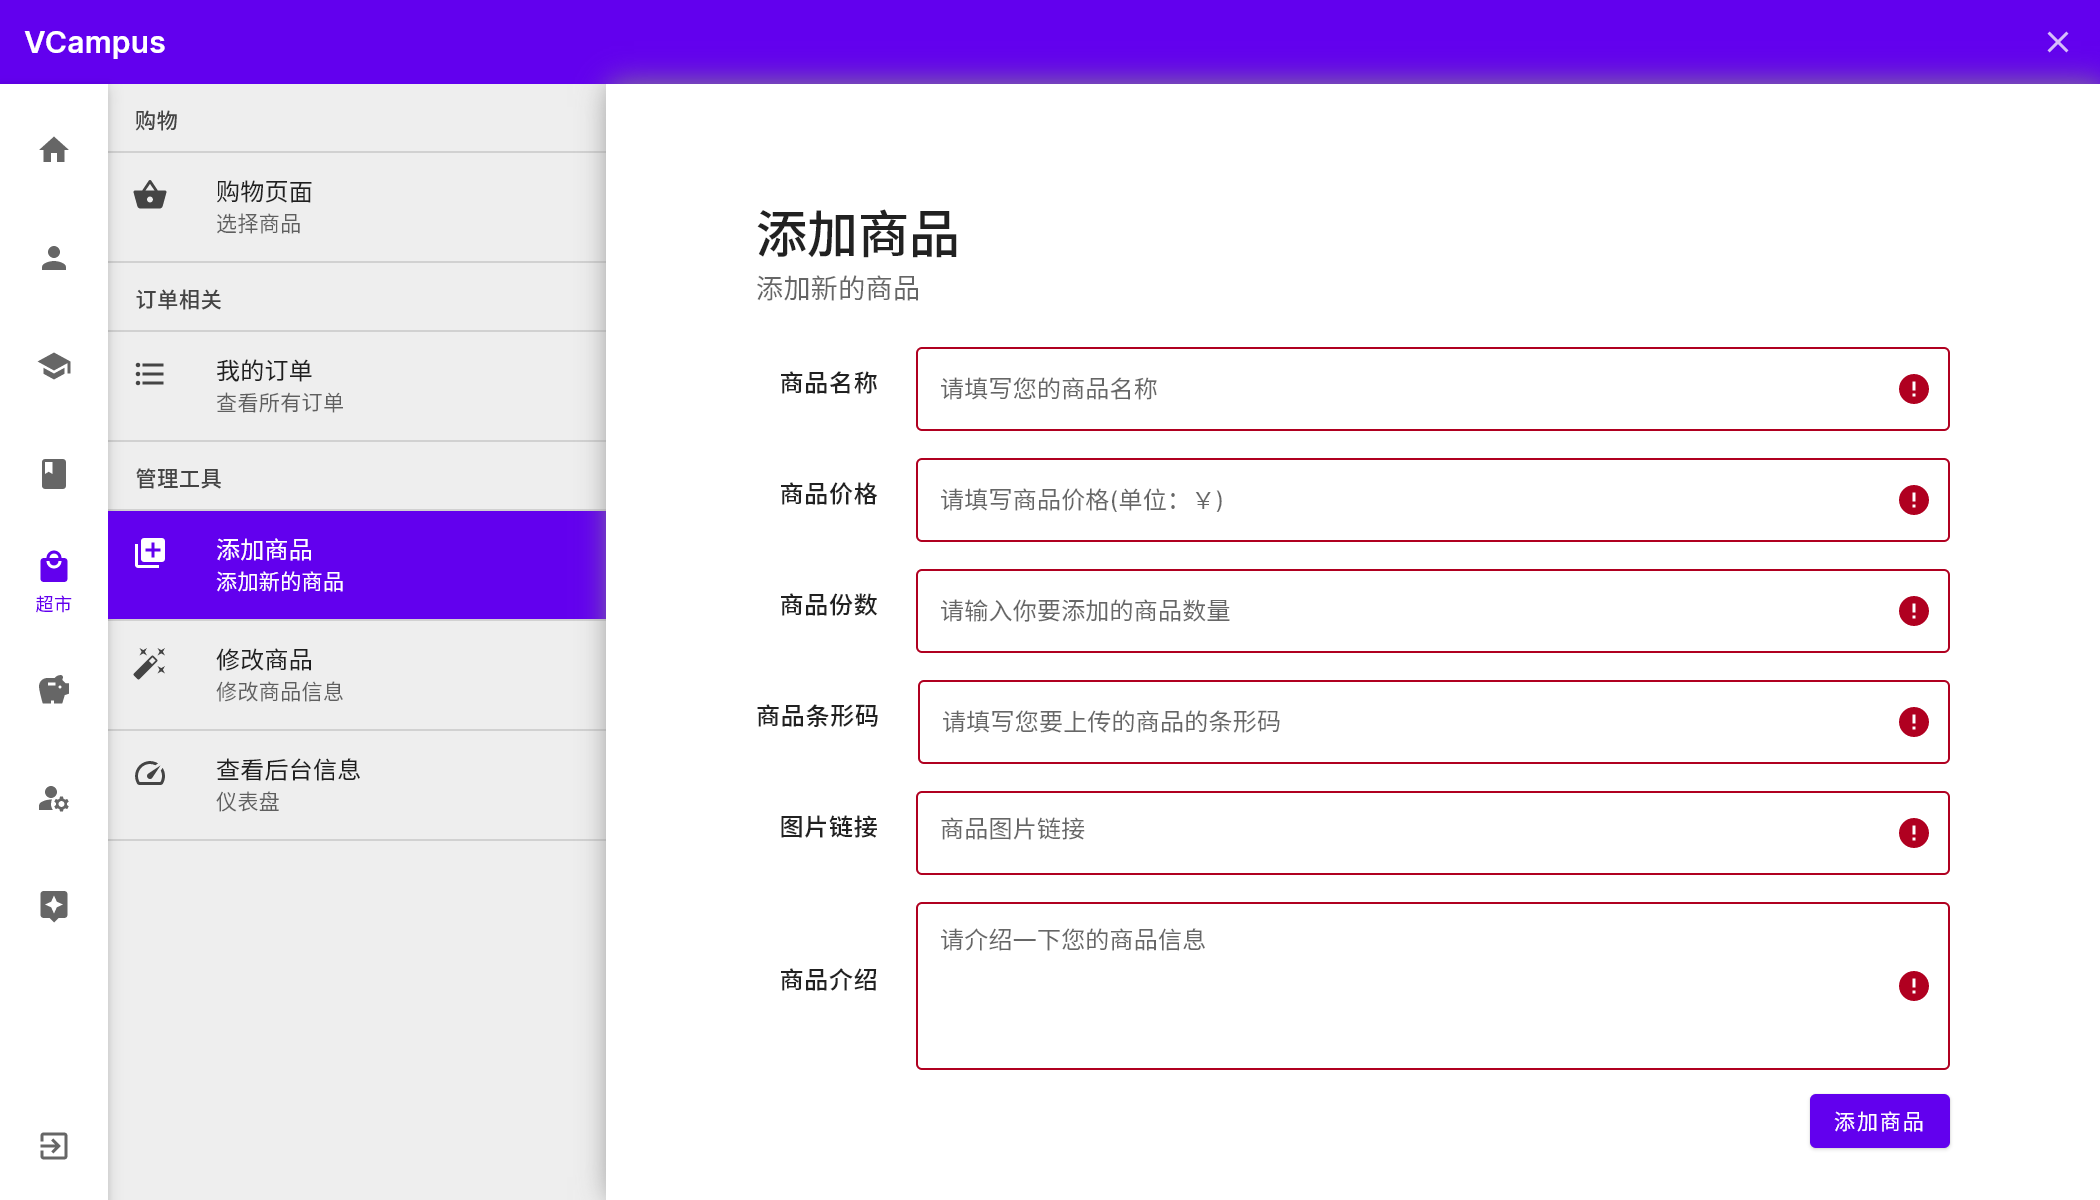
\includegraphics[width=\textwidth]{fig/shop/add_item.png}}
\textbf{商店添加商品信息}
\end{center}

\subsubsection{修改商品}

修改商品界面是商店管理员的管理界面。界面展示了所有的商品条目,点击想要修改的商品条目就可以对商品信息进行修改。也可以在界面上方的搜索框输入关键词,直接搜索到对应的商品,搜索支持模糊查询。

\begin{center}
\shadowbox{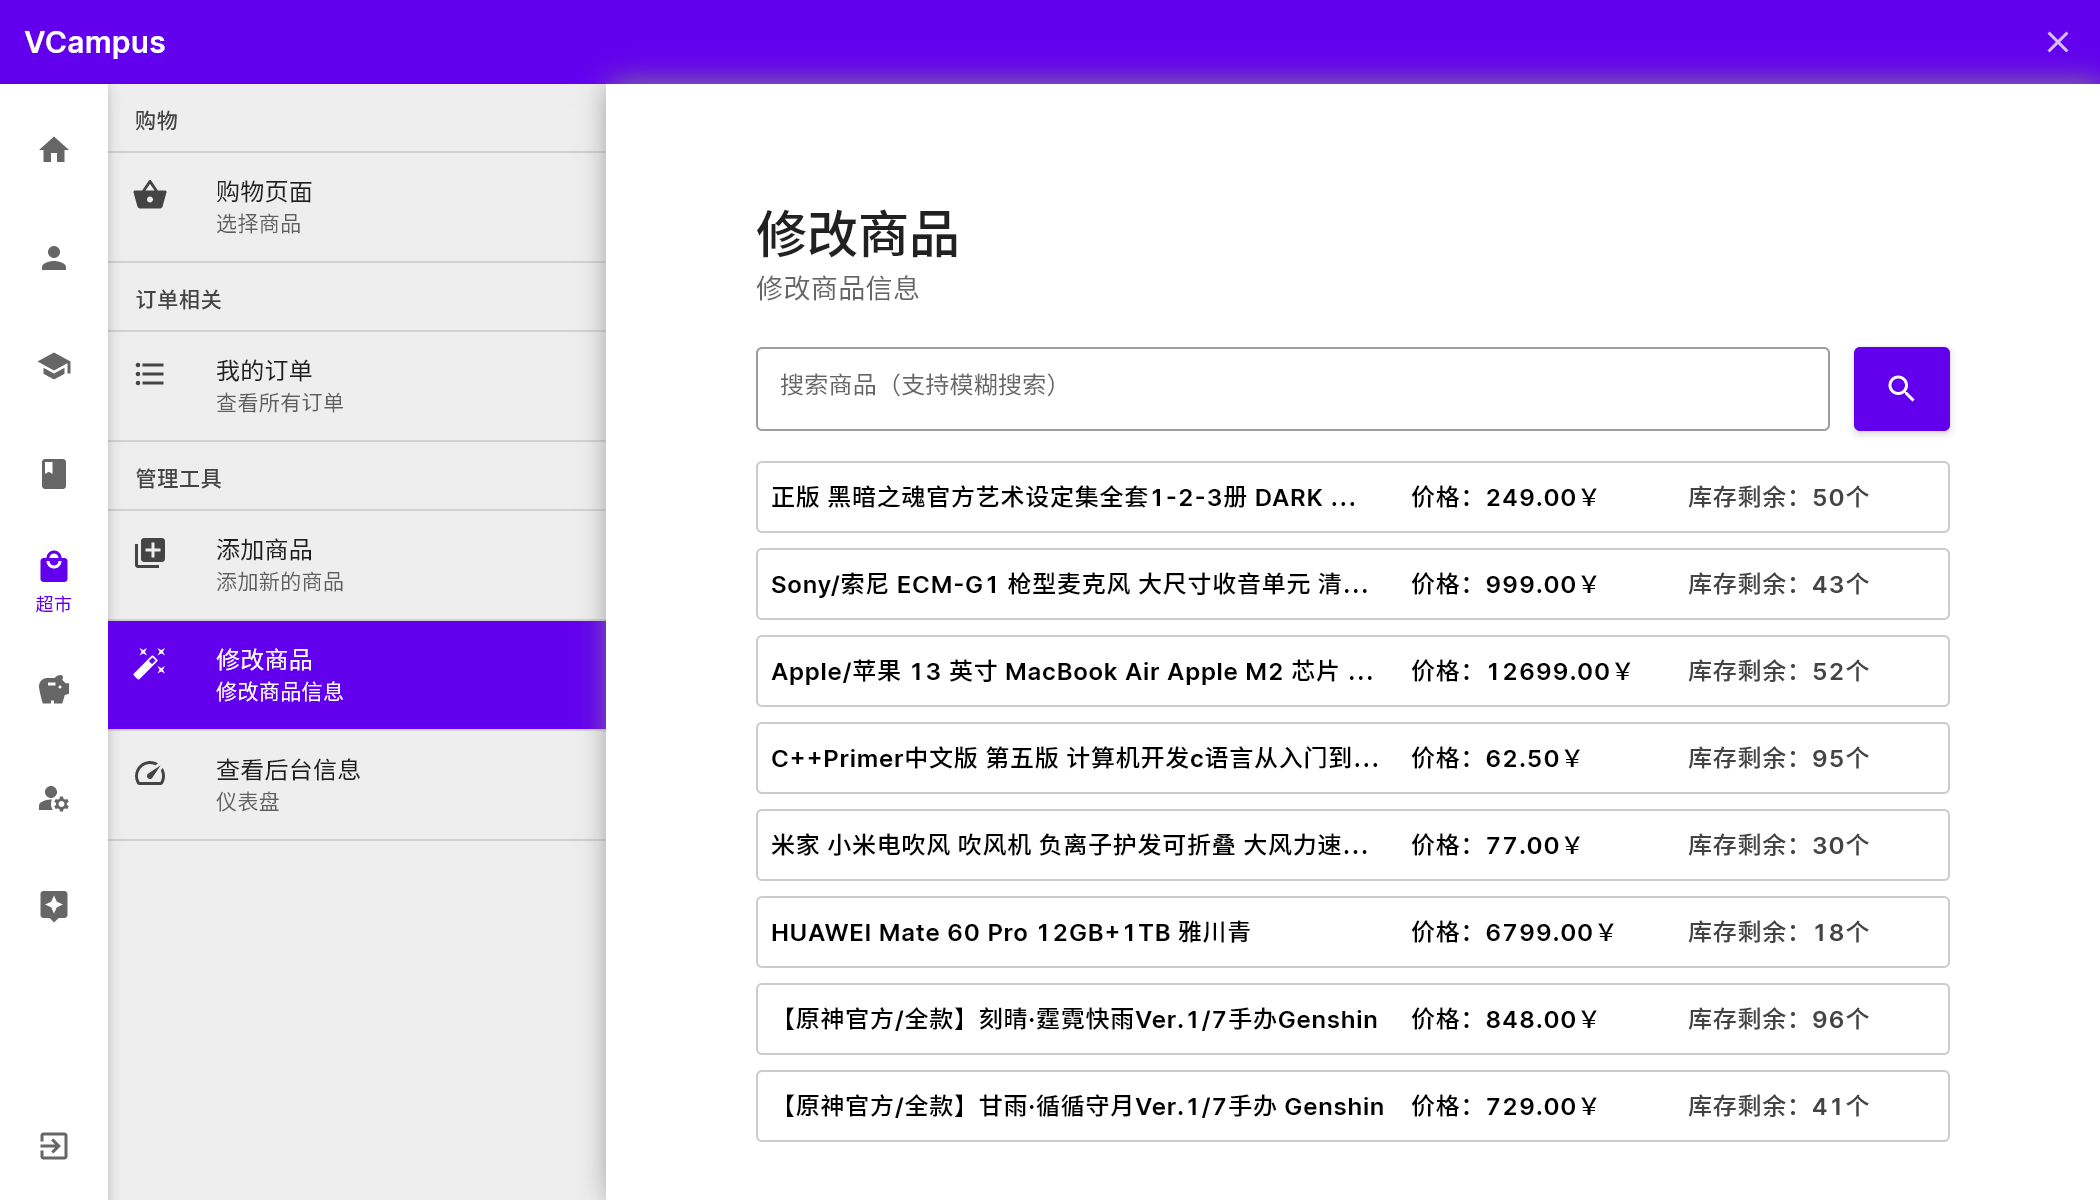
\includegraphics[width=\textwidth]{fig/shop/modify_item.png}}
\textbf{商店修改商品信息}
\end{center}


\subsubsection{查看后台信息}
查看后台信息界面是商店管理员的管理界面。界面展示了所有商品的销售情况(销售额,库存)、以及商品图片、名称、价格等基本信息,同时在这个模块,管理员也可以查看今日的总销售额。



\begin{center}
\shadowbox{\includegraphics[width=\textwidth]{fig/shop/my_bills.png}}
\textbf{商店后台信息}
\end{center}


\subsection{财务}

\subsubsection{一卡通}
学生登录Vcampus后,可以进入这个功能模块查看自己当前的一卡通余额,以及自己近期的账单(包括商店消费减少的金额以及一卡通充值后加入的金额)
\begin{center}
\shadowbox{\includegraphics[width=\textwidth]{fig/finance/my_bills.png}}
\textbf{一卡通余额}
\end{center}

\subsubsection{一卡通管理}
一卡通管理人员登录Vcampus后,可以进入管理模块搜索查看修改一卡通的状态/金额。我们提供了一个搜索框,支持通过一卡通号索引,索引成功后会在搜索框下显示一卡通的相关信息,你可以在这个页面更改一卡通的状态,给一卡通充值金额等操作。
\begin{center}
\shadowbox{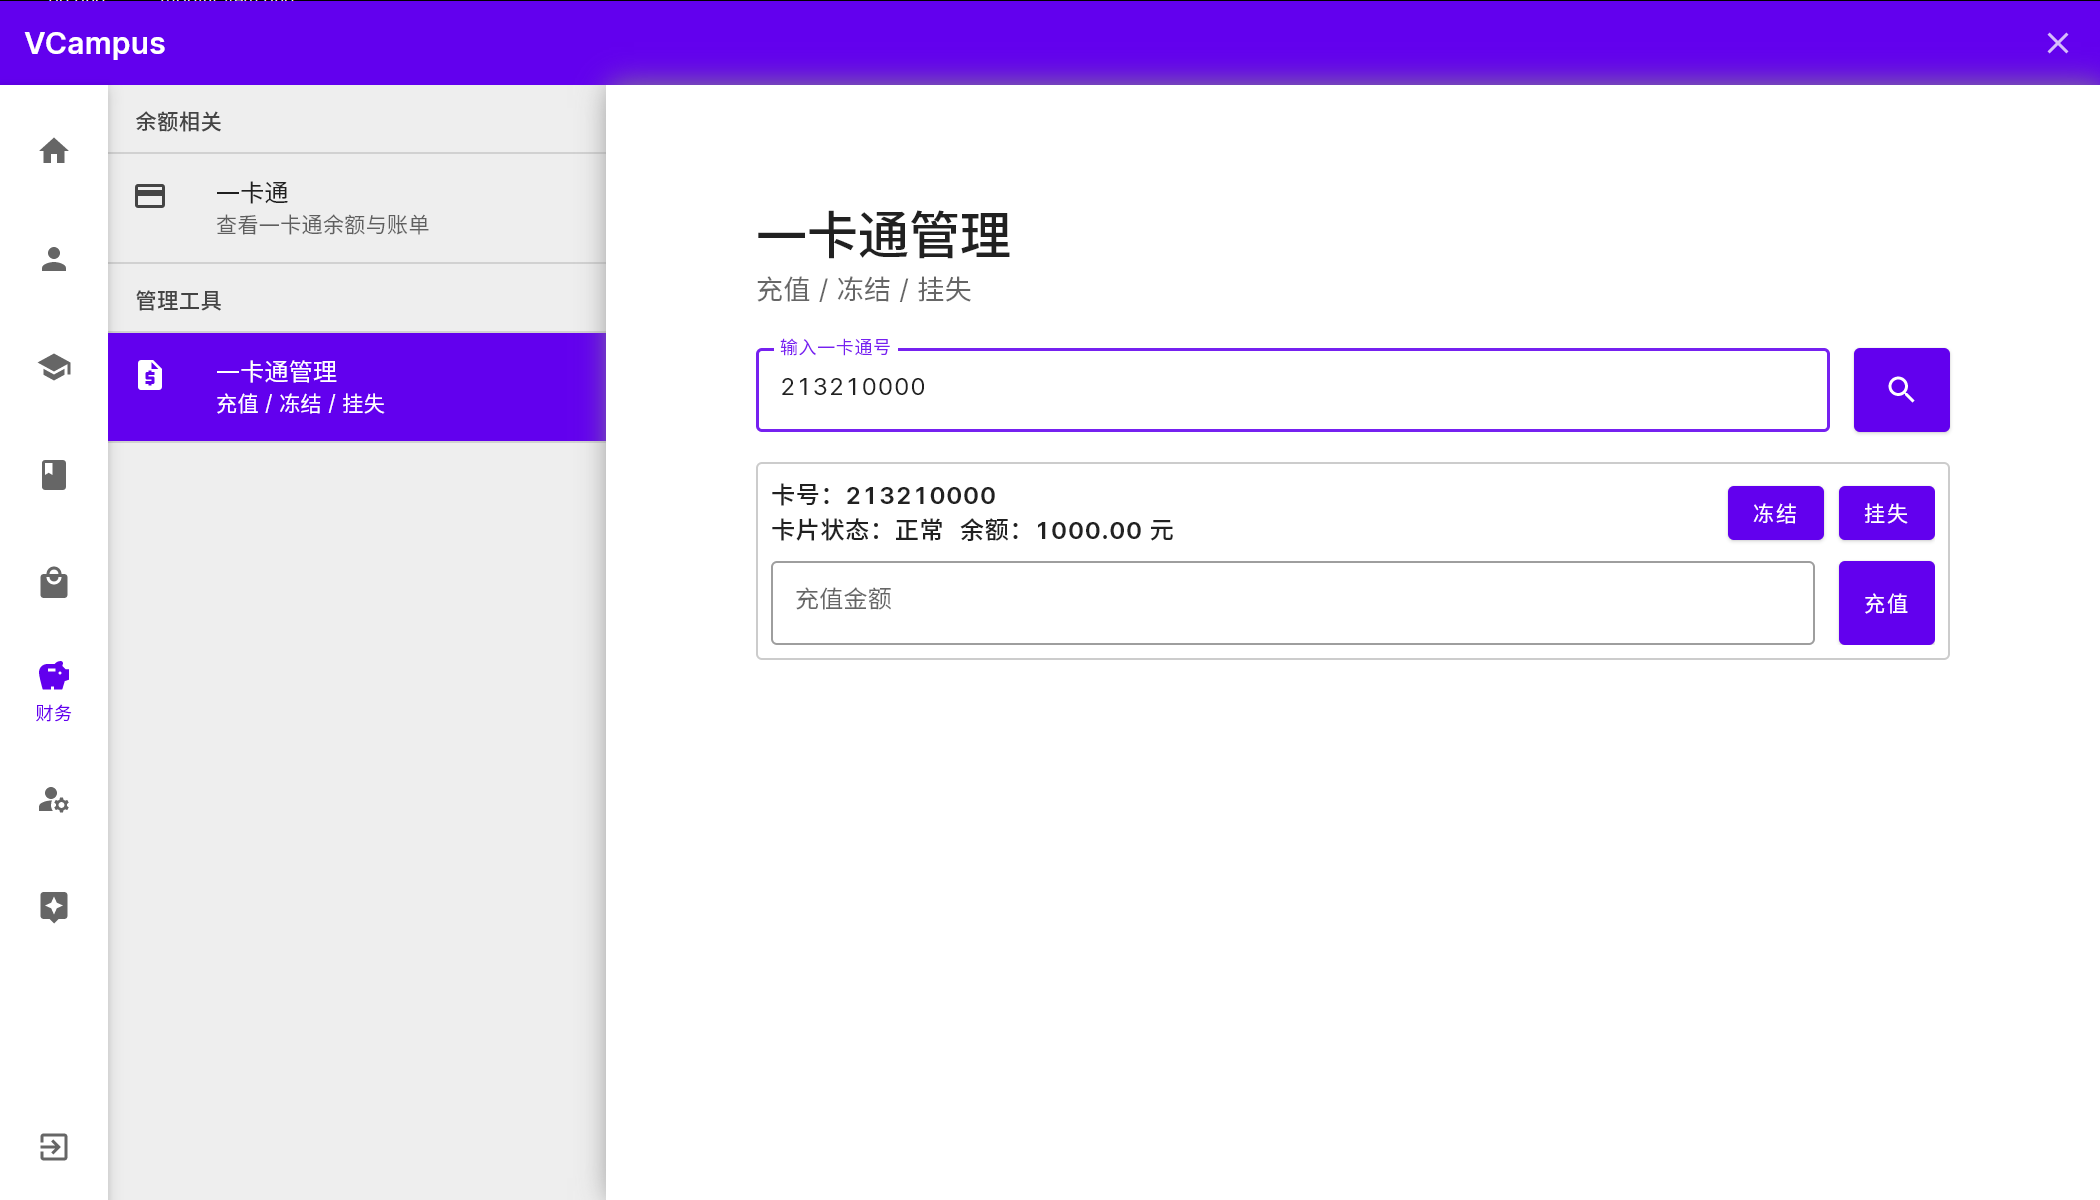
\includegraphics[width=\textwidth]{fig/finance/card_manage.png}}
\textbf{一卡通管理}
\end{center}

\subsection{管理员}

\subsubsection{添加账户}
管理员登录vcampus后,可以进入添加登录账户的页面,在这个页面管理员可以设置新增的一卡通号及初始密码,同时设置姓名、性别、电话、邮箱等基本信息,在最下方的选择栏,管理员可以通过勾选相关职责限制新增用户的不同权限。
\begin{center}
\shadowbox{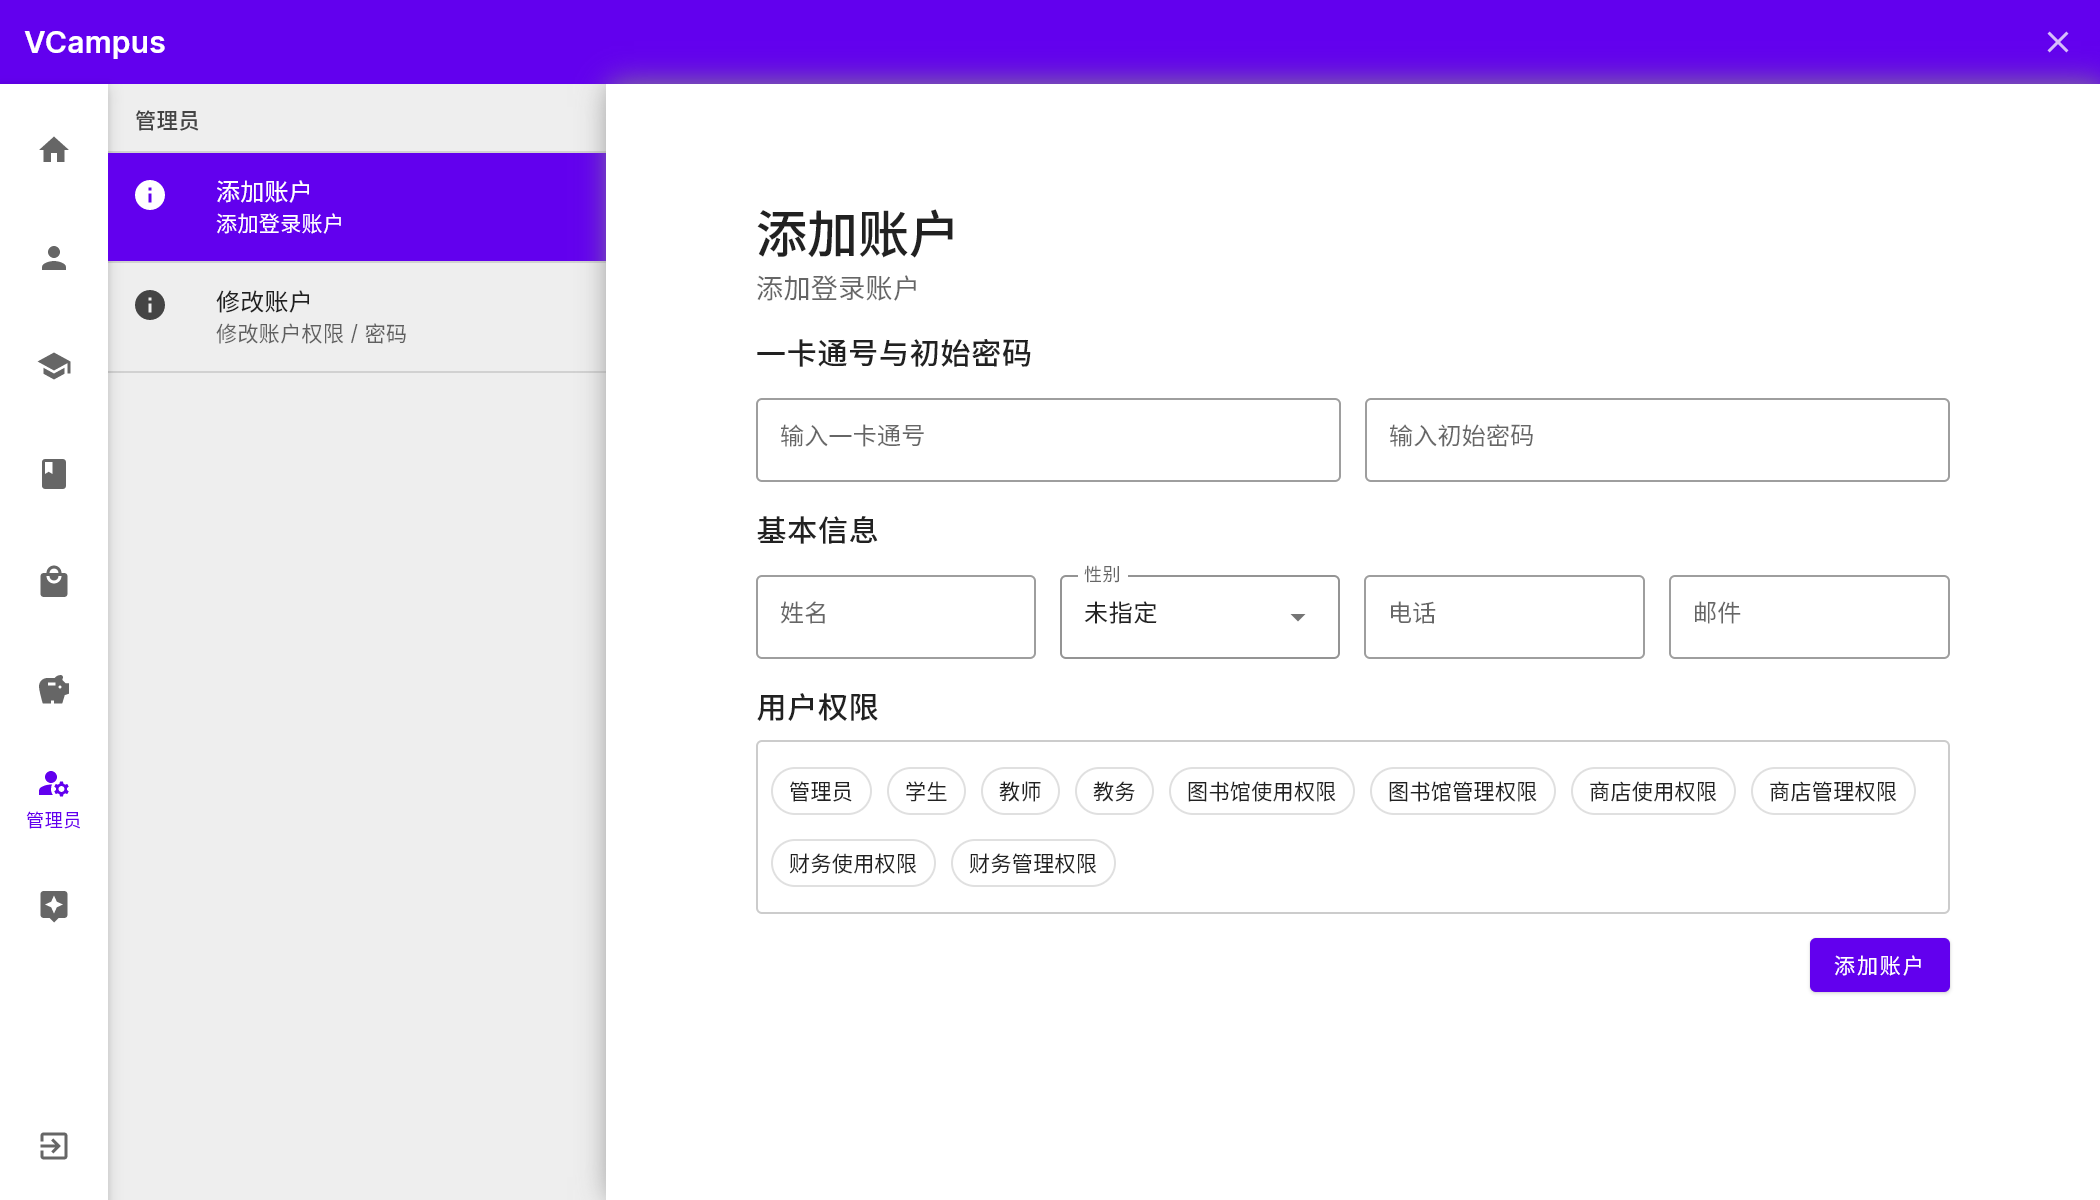
\includegraphics[width=\textwidth]{fig/admin/add_user.png}}
\textbf{管理员添加账户}
\end{center}


\subsubsection{修改账户}
管理员登录vcampus后,可以进入修改账户的界面。当管理员进入该界面后,管理员首先会看到目前已有的所有一卡通号以及他们对应的职责,之后可以点击编辑按钮进行密码(密码输入框不输入则不修改)、权限的修改(通过点击职责按钮来实现)。

\begin{center}
\shadowbox{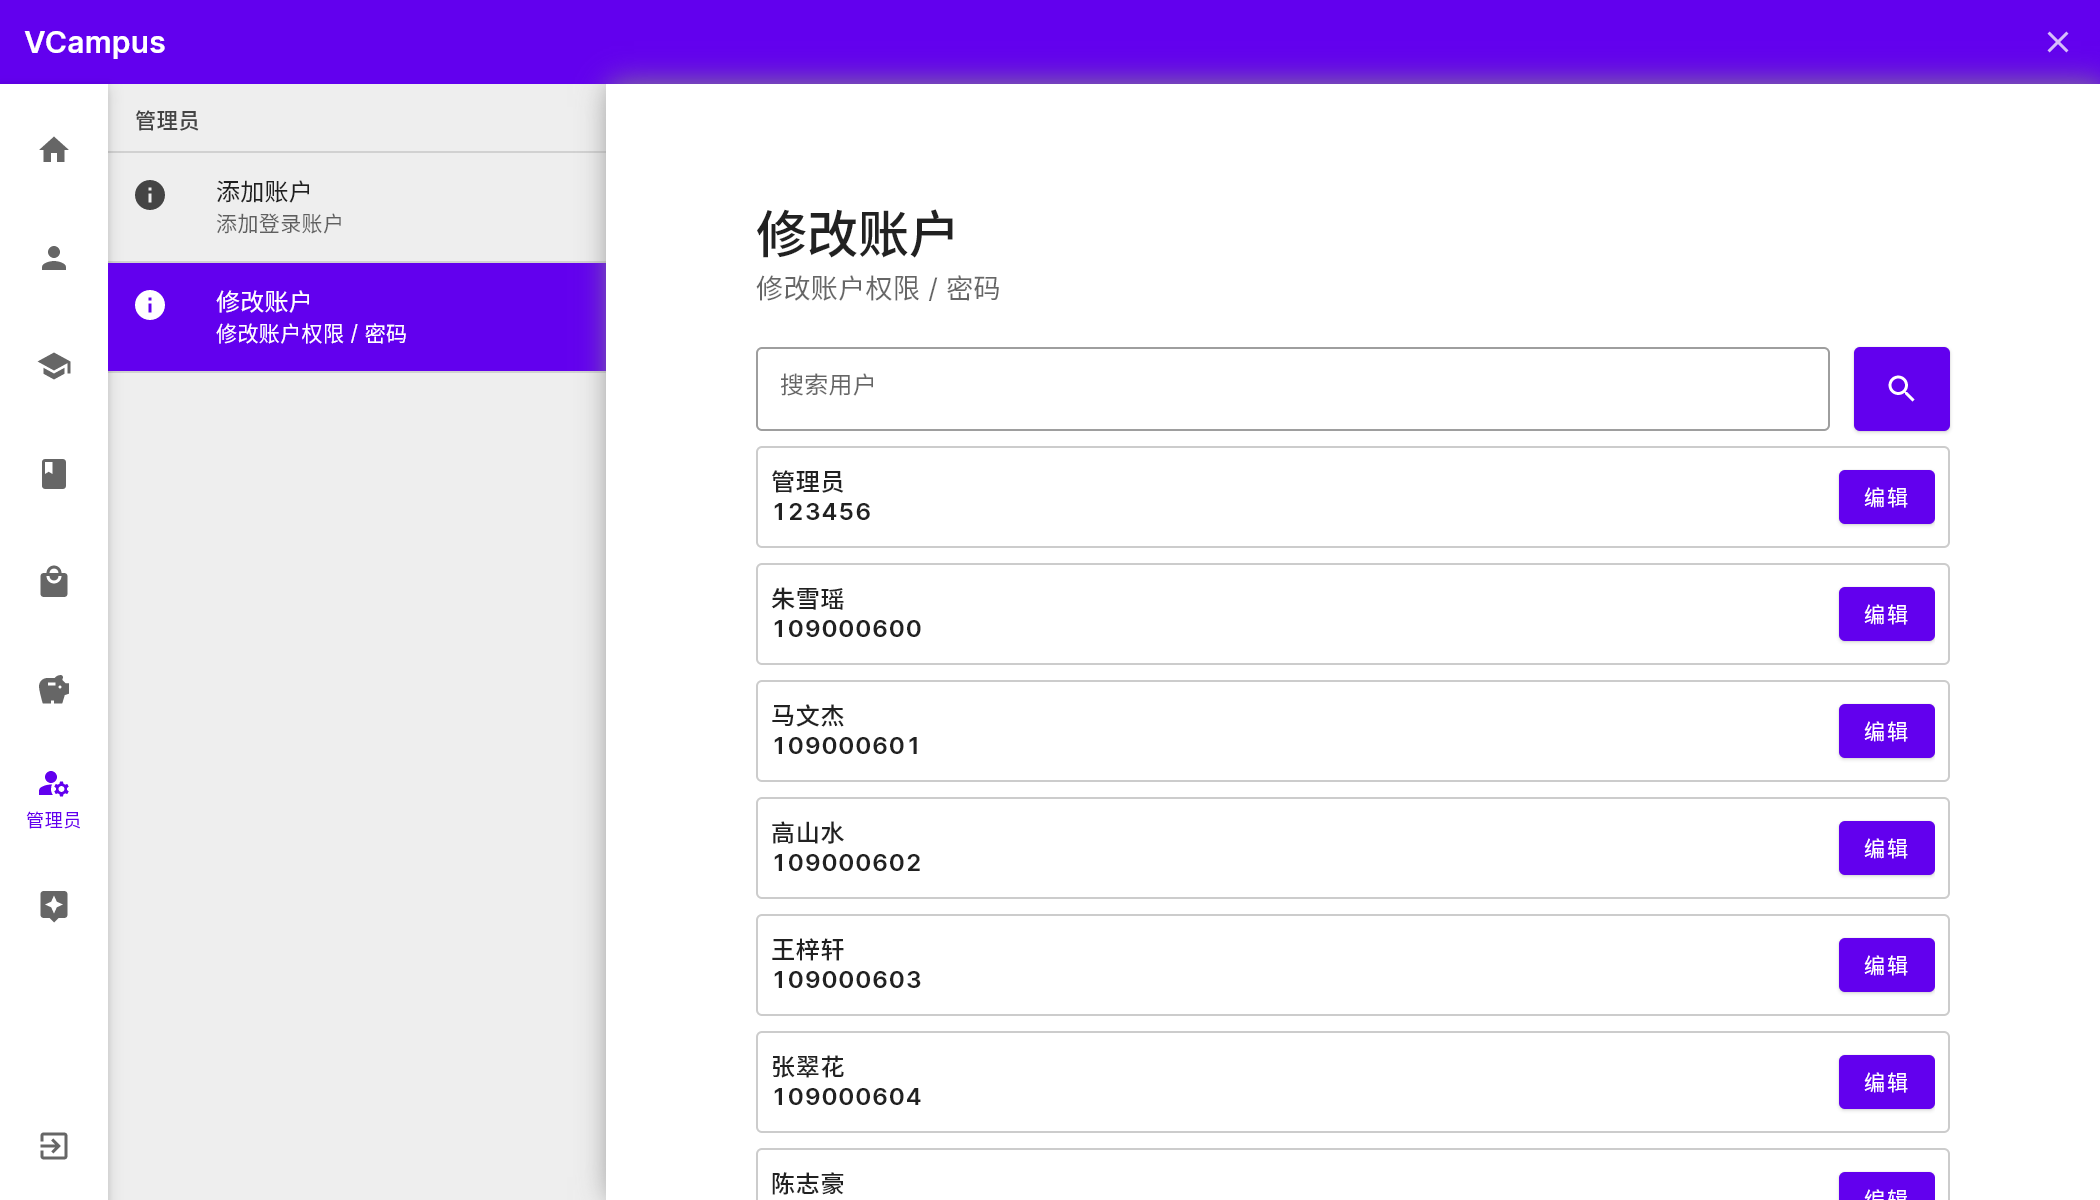
\includegraphics[width=\textwidth]{fig/admin/user_manage.png}}
\textbf{修改账户界面}
\end{center}

\subsection{GPT}
通过这个功能模块,我们给登录Vcampus的师生提供chatgpt-4.0的接口服务,学生们可以通过这个页面与AI进行沟通以及答疑。
\begin{center}
\shadowbox{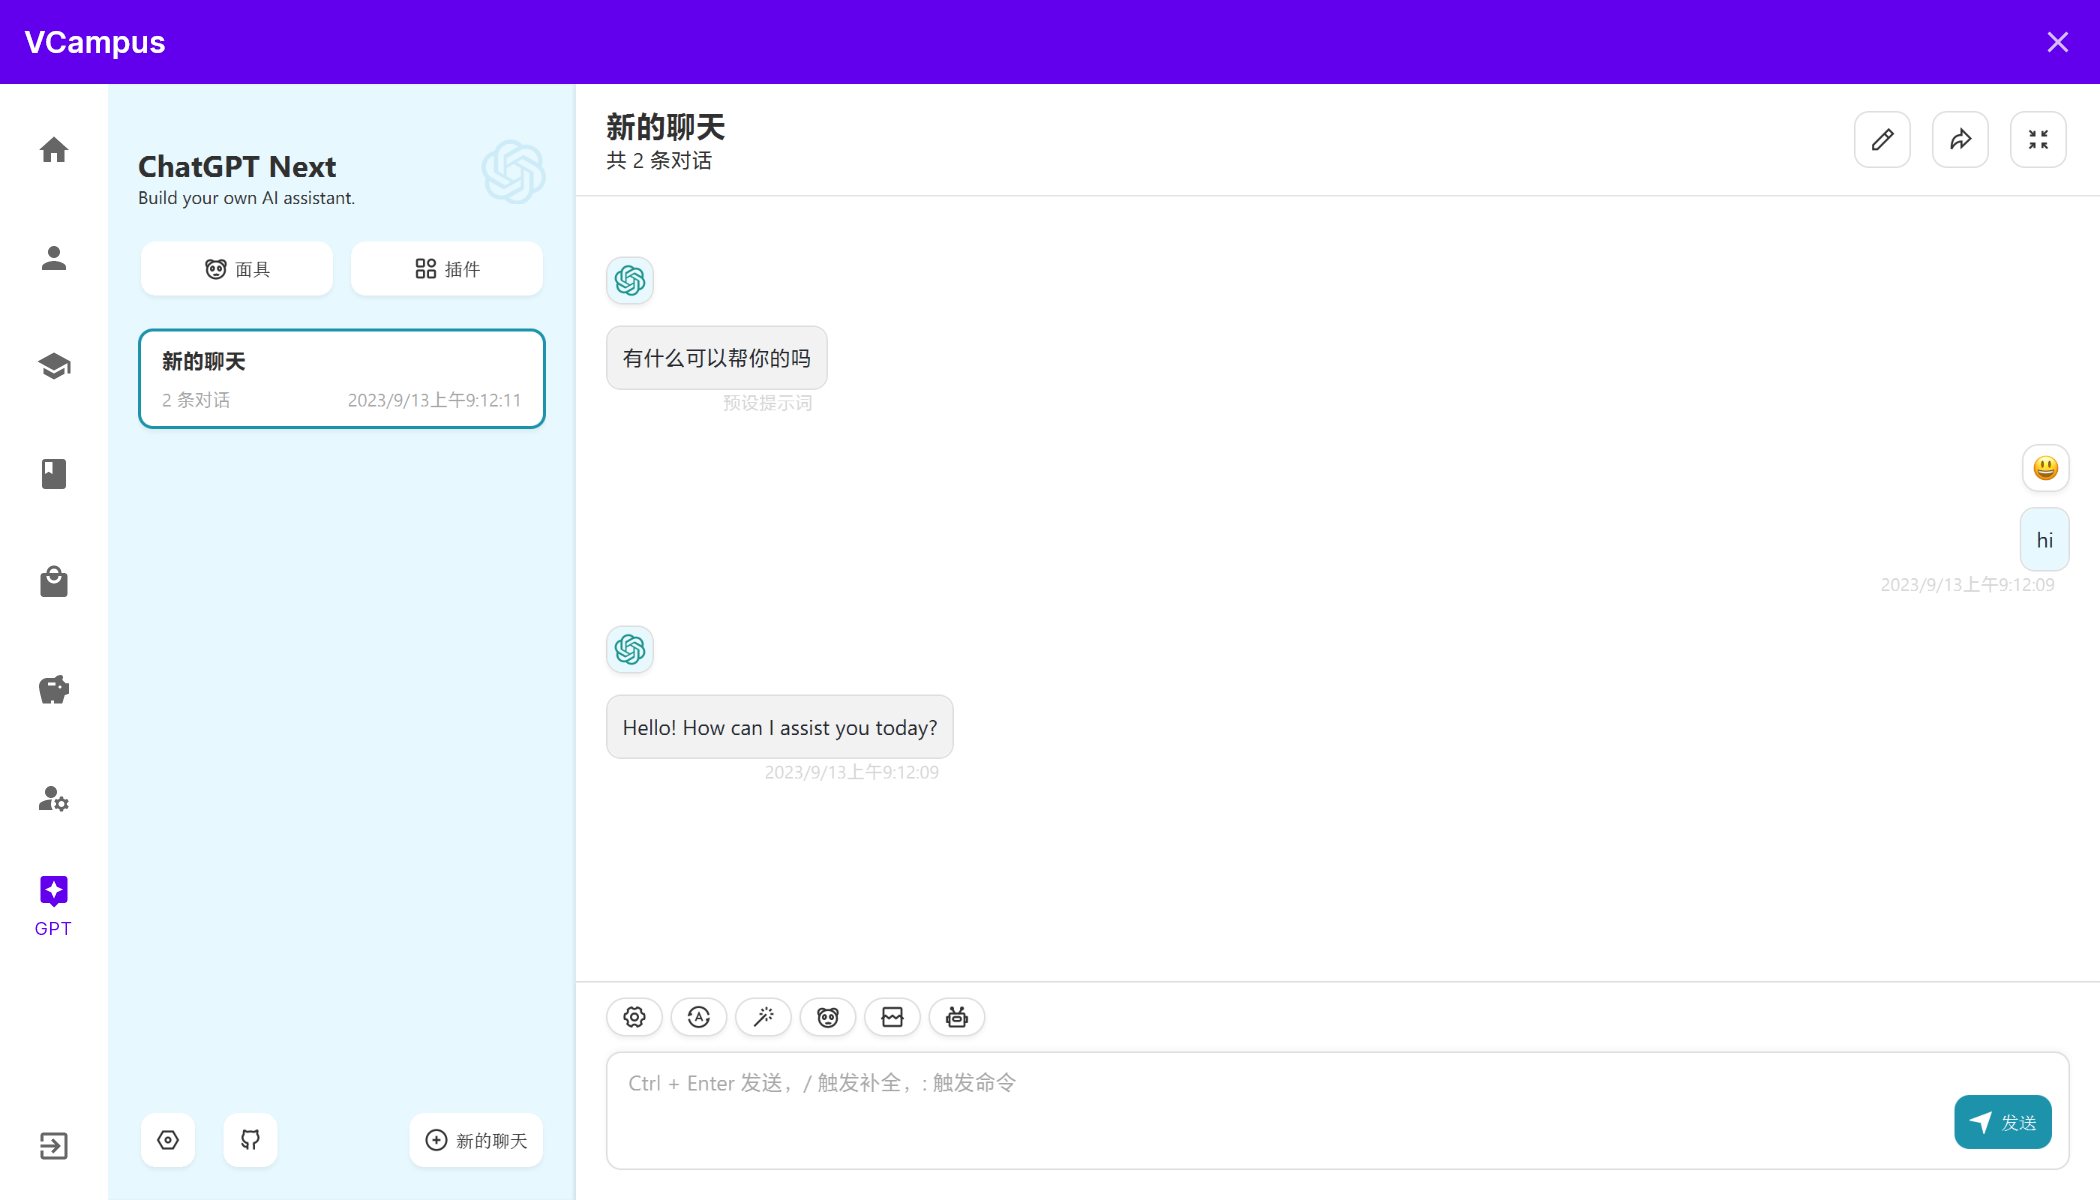
\includegraphics[width=\textwidth]{fig/gpt/gpt.png}}
\textbf{GPT界面}
\end{center}

\end{document}
